\documentclass{beamer}
%
% Choose how your presentation looks.
%
% For more themes, color themes and font themes, see:
% http://deic.uab.es/~iblanes/beamer_gallery/index_by_theme.html
%
\mode<presentation>
{
  \usetheme{default}      % or try Darmstadt, Madrid, Warsaw, ...
  \usecolortheme{lily} % or try albatross, beaver, crane, ...
  \usefonttheme{professionalfonts}  % or try serif, structurebold, structureitalicserif, structuresmallcapsserif
  \setbeamertemplate{navigation symbols}{}
  \setbeamertemplate{caption}[numbered]
} 
%Tables
 \usepackage{booktabs}
\usepackage{multirow}
\usepackage{graphicx}
\usepackage{booktabs}

\usepackage{tikz}

% Define the headline with all section titles
\definecolor{myblue}{RGB}{0, 102, 204}
\usepackage{amssymb}
\setbeamertemplate{headline}{
  \begin{beamercolorbox}[wd=\paperwidth,ht=2.5ex,dp=1ex,center]{palette primary}
    {\color{myblue} \tiny 
    \only<1->\insertsectionnavigationhorizontal{\paperwidth}{}{}}
  \end{beamercolorbox}
}

% Apply colors to the block
\usepackage[dvipsnames]{xcolor}
% Define custom colors
\definecolor{blockbg}{RGB}{230, 240, 255}  % Light blue background
\definecolor{blockborder}{RGB}{0, 102, 204} % Dark blue border
\definecolor{blocktitle}{RGB}{255, 255, 255} % White title text
\setbeamercolor{block title}{fg=blue, bg=white}
\setbeamercolor{block body}{bg=blockbg}

% Add page number at the bottom right
\setbeamertemplate{footline}{
  \hfill
  \usebeamercolor[fg]{page number in head/foot}
  \usebeamerfont{page number in head/foot}
  \insertframenumber/\inserttotalframenumber
  \hspace{1em}
}

\usepackage[english]{babel}
\usepackage[utf8]{inputenc}
\usepackage[T1]{fontenc}

\usepackage{caption}
\usepackage{tikz}

\usepackage{xcolor}

\title[Economic Shocks, Retirement \& Mental Health]{How Do Economic Shocks Impact Upon the Mental Health of Retirees?}
\author{Mario Martínez-Jiménez}
\institute{Imperial College Business School}
\date{\footnotesize March 12, 2025\\
\vspace{0.45cm}
ISER, University of Essex}

\begin{document}

\begin{frame}
\thispagestyle{empty}  % Remove page number
  \setbeamertemplate{headline}{}  % Remove headline
  \titlepage
\end{frame}


\small
\begin{frame}{Why is it important?}
\footnotesize
\begin{enumerate}
\footnotesize
\item<1-> The population in high-income countries is \begingroup\color{Blue}ageing rapidly \endgroup

 \begin{itemize}
 \scriptsize
    \item 	Rise from 17.6\% of the UK population was aged 65 or older in 2014 to 19\% by 2022 - projected to rise to 27\% by 2027 (\begingroup\color{lightgray}ONS, 2024\endgroup)
\end{itemize}

\vspace{0.3cm}

\item<2->	Older adults often face \begingroup\color{Blue}health challenges \endgroup and major life transitions that heighten their risk of mental health conditions  \scriptsize{(\begingroup\color{lightgray}CDC Healthy Aging, 2024\endgroup)}

 \begin{itemize}
 \scriptsize
    \item 	\begingroup\color{Blue}Macroeconomic shocks  \endgroup are now more frequent which might influence retirees' mental health and well-being 
\end{itemize}

\vspace{0.3cm}

\item<3-> Understand the challenges associated with the ageing population and  \begingroup\color{Blue}increasing prevalence of mental health \endgroup issues among retirees 

\begin{itemize}
 \scriptsize
    \item 	Approximately 14\% of adults aged 60 and over live with a \begingroup\color{Blue}mental disorder  \endgroup \scriptsize{(\begingroup\color{lightgray}Global Health Estimates, 2019\endgroup)}
\end{itemize}


\end{enumerate}

\end{frame}


\begin{frame}{Why is it important?}
    \framesubtitle{Policy \& Socially relevant}
\footnotesize
\begin{center}
   %  \vspace*{1cm}  % Adjust the vertical space for centering
    \begin{tikzpicture}
      % Center the first image in the middle of the frame
      \node[anchor=center] (img1) at (0, 0) {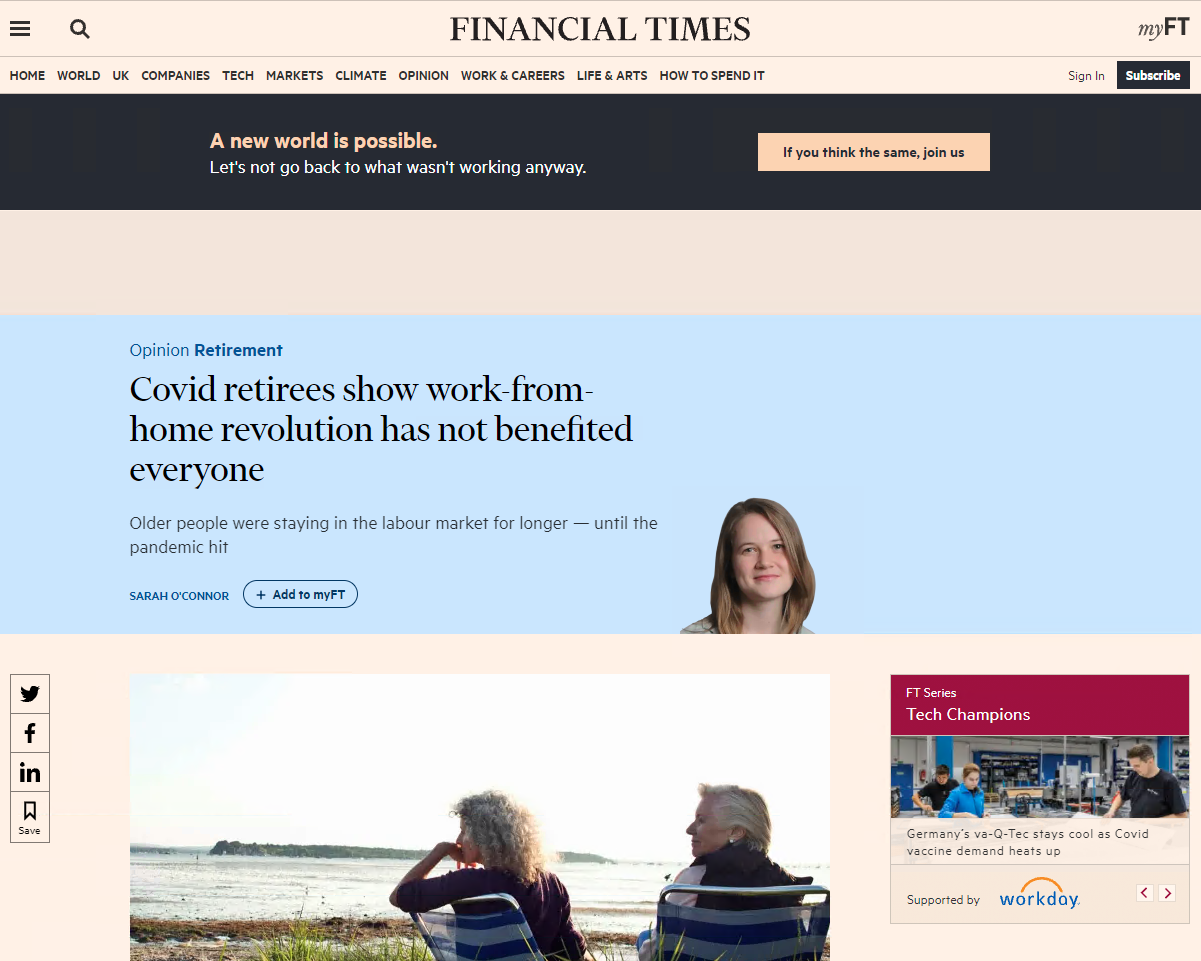
\includegraphics[height=7.5cm]{picFT.png}};
      \pause
      \node (img2) at (img1.south east) [yshift=6.5cm] {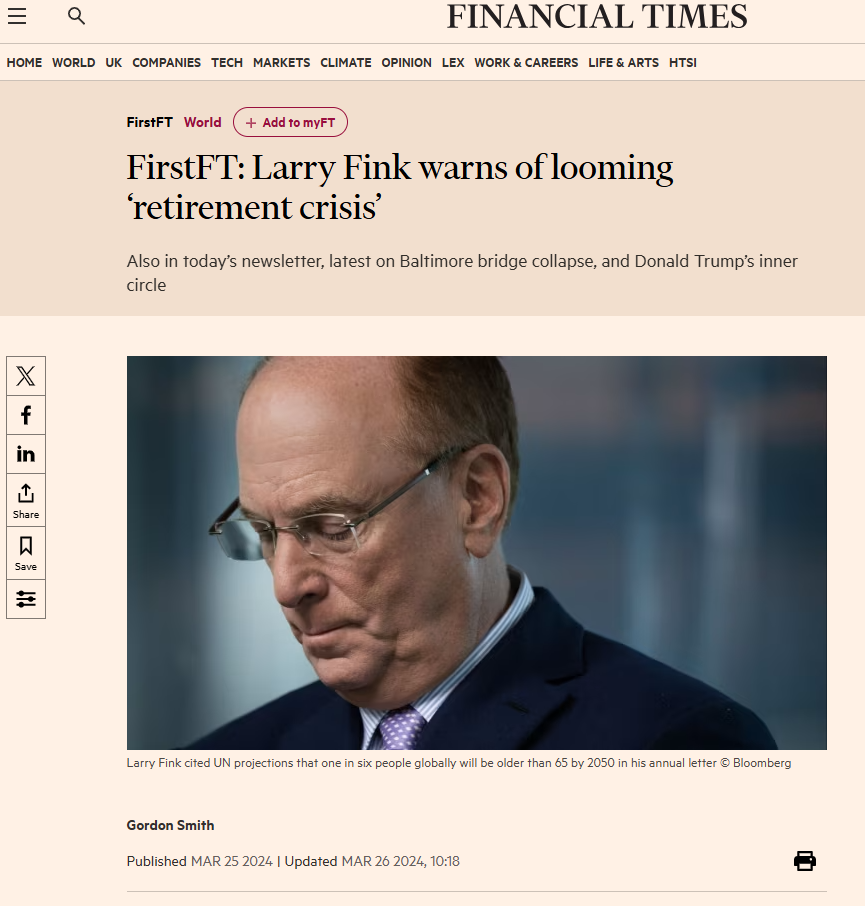
\includegraphics[height=7.5cm]{picFT_2.png}};
      \pause
      \node (img3) at (img2.south west) [yshift=3.5cm] {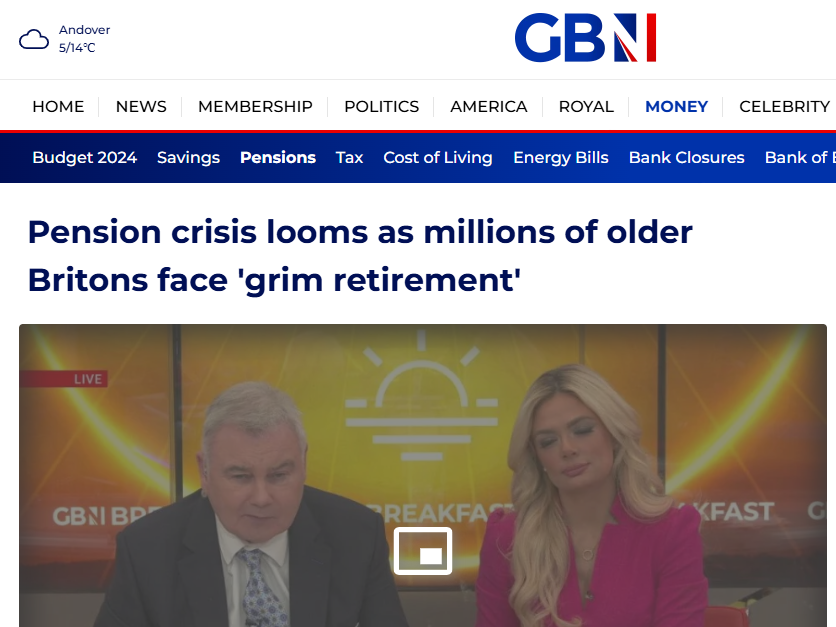
\includegraphics[height=7cm]{GBN_news.png}};
    \end{tikzpicture}
  \end{center}

\end{frame}



\begin{frame}{Research Question}

  % Block with the research question (appears first)
  \begin{block}{}
    \centering
    \textbf{Question 1:} Is retirement good for mental health and well-being? 
  \end{block}

  \vspace{0.5cm}   

  % Images appear in one row, progressively
  \begin{figure}[H]
    \centering
    \begin{minipage}{.5\textwidth}
      \centering
      \only<2->{
\includegraphics[width=.85\linewidth, height=100px]{Pic2.jpg}}
    \end{minipage}%
    \begin{minipage}{.5\textwidth}
      \centering
      \only<3->{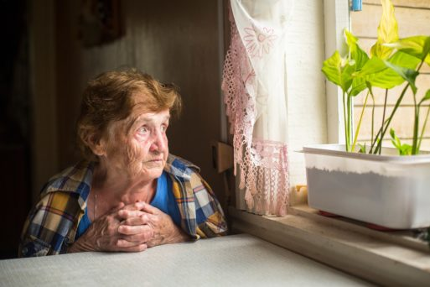
\includegraphics[width=.85\linewidth, height=100px]{Picture_1.png}}
    \end{minipage}
  \end{figure}

\end{frame}


    
  \begin{frame}{Research Questions}
    
  % Block with the research question (appears first)
  \begin{block}{}
    \centering
    \textbf{Question 2:} Can economic shocks influence the mental health effects of retirement?
  \end{block}

  \vspace{0.5cm}   

  % Images appear in one row, progressively
  \begin{figure}[H]
    \centering
    \begin{minipage}{.5\textwidth}
      \centering
      \only<2->{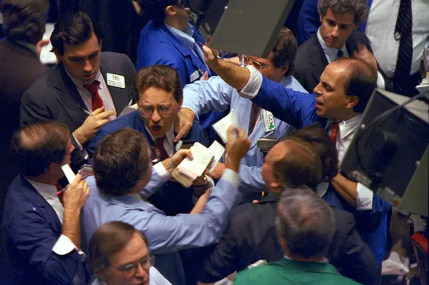
\includegraphics[width=.85\linewidth, height=100px]{P3.png}}
    \end{minipage}%
    \begin{minipage}{.5\textwidth}
      \centering
      \only<3->{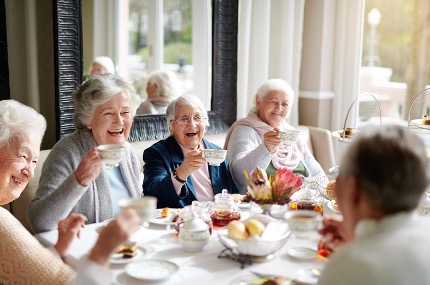
\includegraphics[width=.85\linewidth, height=100px]{P4.jpg}}
    \end{minipage}
  \end{figure}
    
\end{frame}


\begin{frame}{Contributions}
    \footnotesize
\begin{itemize}
    \item<1-> Several studies suggest that changes in \begingroup\color{Blue}labour market conditions \endgroup may affect mental health with \textbf{conflicting results} \scriptsize{(\begingroup\color{lightgray}Ruhm 2000 \endgroup v.s. \begingroup\color{lightgray}Ruhm 2015\endgroup)}
\begin{itemize}
\scriptsize
    \item<2-> \textbf{Negative} effects via \textit{uncertainty, financial stress, loss of employment, insurance}
    
\item<3-> \textbf{Positive} effects via \textit{less unhealthy behaviour}
\end{itemize}
\footnotesize
    \vspace{0.3cm}
    \item<4->  \textbf{No work} yet on mental health effect of retirement during a financial shock in the \begingroup\color{Blue}United Kingdom\endgroup:
    
    \begin{itemize}
    \scriptsize
    \item<5-> \textbf{Escape} from rapidly deteriorating labour market conditions (\begingroup\color{Blue}work-related stress/strain\endgroup)
    \item<6->  \begingroup\color{Blue}Reliance on market-dependent pensions \endgroup amplifies the financial strain on retirees during recessions%, offering a unique context to assess the health impacts of retirement in economic crises. 
   
 \end{itemize}
  \vspace{0.25cm}
\footnotesize
 \item<7-> Only \begingroup\color{Blue}one \endgroup previous article has addressed this relationship:

 
   \vspace{0.15cm}
   
    \begin{enumerate}[$\Rightarrow$]
    \scriptsize
        \item<7->  \begingroup\color{lightgray}Belloni et al. (2016) \endgroup  find that retiring immediately after an economic shock improves mental health, although only among blue-collar men living in the most severely affected regions (in \begingroup\color{Blue}10 European countries\endgroup)
   \end{enumerate}
    
\end{itemize}   
\end{frame}

% Uncomment these lines for an automatically generated outline.
\begin{frame}{Outline}
 \tableofcontents
\end{frame}

\section{Overview \& Data}

\begin{frame}{This Paper: Aims}

\footnotesize
\begin{block}{}
\centering
To what extent do severe economic shocks influence the mental health effects of retirement?

\end{block}

   \vspace{0.25cm}
  
\begin{enumerate}

\footnotesize
\item<2-> Estimate the effects of \begingroup\color{Blue}retirement \endgroup on \begingroup\color{Blue}well-being \endgroup and \begingroup\color{Blue}mental \endgroup health of retirees

   \vspace{0.25cm}
   
\item<3-> Explore whether \begingroup\color{Blue}retiring in regions severely impacted by economic crises  \endgroup alters retirees' mental health and well-being outcomes

   \vspace{0.25cm}
   
\item<4-> Consider a set of potential \begingroup\color{Blue}mechanisms  \endgroup  driving this relationship (including financial conditions, age at retirement, health behaviours and social circumstances)
\end{enumerate}


\end{frame}

\begin{frame}{This Paper: Methodology}

\begin{block}{}
\footnotesize
\centering
We employ two \textbf{causal inference methods} to data from English Longitudinal Study of Ageing (2002–2019)
\end{block}

   \vspace{0.25cm}
  
\begin{itemize}
\footnotesize

 \item<2-> English \begingroup\color{Blue}panel \endgroup data for individuals aged 50+ from eight waves of the \begingroup\color{Blue}English Longitudinal Study of Ageing (ELSA)\endgroup
 
   \vspace{0.25cm}
  
\item<3-> We implement \begingroup\color{Blue}fixed effect (FE) \endgroup and \begingroup\color{Blue}instrumental variables fixed-effects (IV-FE) \endgroup approaches 

   \vspace{0.25cm}
  
\item<4-> Regional variation in \begingroup\color{Blue}unemployment rates \endgroup to capture the differential severity of economic shocks
\end{itemize}

\vskip 1cm



\end{frame}


\begin{frame}{This Paper: Preview of Results}

\footnotesize
\begin{block}{}
\centering
How do economic shocks influence the effects of retirement on mental health?
\end{block}

\begin{itemize}

  \item<2-> We find  that the \begingroup\color{Blue}mental \endgroup health effects of \begingroup\color{Blue}retirement  \endgroup are influenced by the presence of \begingroup\color{Blue}economic shocks  \endgroup
\begin{itemize}
\scriptsize
 \setbeamertemplate{itemize subitem}{\textbullet} 
\item<3-> \begingroup\color{Blue}Retirement  \endgroup generally increases the likelihood of experiencing \begingroup\color{Blue}loneliness \endgroup

\item<4-> Retiring in \begingroup\color{Blue}regions severely affected by economic crises  \endgroup reduces the probability of being diagnosed with a \begingroup\color{Blue}psychiatric condition  \endgroup
\end{itemize}

 \item<5-> Our \begingroup\color{Blue}heterogeneous \endgroup analyses: 
 \begin{itemize}
\scriptsize
 \setbeamertemplate{itemize subitem}{\textbullet} 
\item<6-> This \begingroup\color{Blue}short-term  \endgroup mental health benefit is particularly pronounced among \begingroup\color{Blue}men  \endgroup and \begingroup\color{Blue}white-collar workers  \endgroup 
\item<7-> These positive effects \begingroup\color{Blue}diminish over time\endgroup, suggesting that the initial relief from job-related stress is not sustained in the long run


\end{itemize}

 \item<8-> Our \begingroup\color{Blue}mechanism \endgroup analyses: 
 \begin{itemize}
\scriptsize
 \setbeamertemplate{itemize subitem}{\textbullet} 
\item<9-> \begingroup\color{Blue}Financial security\endgroup, \begingroup\color{Blue}healthy lifestyles\endgroup, and the \begingroup\color{Blue}ability \endgroup to retire upon reaching eligibility retirement ages—particularly among white-collar retirees


\end{itemize}
\end{itemize}

\end{frame}



\begin{frame}{Data}
\footnotesize
The \begingroup\color{Blue}English Longitudinal Study of Ageing (ELSA) \endgroup dataset (2002-2019)

\begin{itemize}
\footnotesize
        \item Covers individuals \textbf{aged 50 and over} living in \textbf{England}
        \item \textbf{Biannual} longitudinal panel dataset
        \item A \begingroup\color{Blue}wealth  \endgroup  of health-related data (diagnosed conditions, mental health) and socioeconomic aspects related to employment, wealth and pensions

    \vspace{0.15cm}
    \item<2-> To define \textbf{retirement}: 
\begin{enumerate}
\scriptsize
        \item We pooled everyone who is in \begingroup\color{Blue}paid work \endgroup (employees or self-employed) in first wave (March 2002 – March 2003)
        \item Individual retires from work between \begingroup\color{Blue}consecutive \endgroup waves $\rightarrow$ self-reported labour position as \begingroup\color{Blue}retired \endgroup and no paid work in the last month
\item \textbf{Absorbing state}: \begingroup\color{Blue}first \endgroup exits from the labour market
       
    \end{enumerate}
    
     \vspace{0.3cm}
    \item<3-> \begingroup\color{Blue}Unbalanced \endgroup panel dataset: 
    \begin{itemize}
    \footnotesize
        \item 2,668 individuals
        \item 8,900 observations in \textbf{employed} group and 6,588 \textbf{retirement} group
    \end{itemize}

\end{itemize}
\end{frame}



\begin{frame}{Outcome and control variables}
\footnotesize
\begin{enumerate}

\item<1-> \begingroup\color{Blue}Outcome variables\endgroup:  

\begin{itemize}
\scriptsize
    \item<2-> \textbf{Mental Health} $\rightarrow$ (i) Depression Symptoms [0-8] and (ii) newly diagnosed psychiatric condition (physician-diagnosed depression or anxiety after retirement)

    \item<3-> \textbf{Well-being} $\rightarrow$ (i) Feeling lonely and (ii) life satisfaction
\end{itemize}

\item<4-> \begingroup\color{Blue}Heterogenous analyses \endgroup $\rightarrow$  gender, white-collar vs blue-collar, and \begingroup\color{Blue}short- (2004-2013)  \endgroup vs \begingroup\color{Blue}long-term (2004-2019) \endgroup

\item<5-> \begingroup\color{Blue}Mechanism analyses: \endgroup 

 \begin{itemize}
\scriptsize
 \setbeamertemplate{itemize subitem}{\textbullet} 
\item<6->\textbf{Financial security}$\rightarrow$ BU Net Financial Wealth (top quartile)
\item<7-> \textbf{Social isolation}$\rightarrow$ Live with at least one adult or child 
\item<8-> \textbf{Flexible retirement option}$\rightarrow$ Retirement age before SPA
\item<9-> \textbf{Healthy behaviours}$\rightarrow$ Physical activity (moderate/vigorous)
\end{itemize}

\item<10-> \begingroup\color{Blue}Control variables\endgroup: 
 \begin{itemize}
\scriptsize
 \setbeamertemplate{itemize subitem}{\textbullet} 
\item<11-> Age, age squared, gender, marital status, household size, tenure, private pension, total state pension income, current smokers, physical activity and health insurance

\item<12->  \textbf{Region} characteristics (multiple deprivation index and population density quintiles by postcode) and \textbf{time} FE
\end{itemize}

\end{enumerate}
\end{frame}   




\section{Empirical Strategies}

\begin{frame}{Empirical Strategies (I): Panel FE}
\footnotesize

 The first and simplest model is a \begingroup\color{Blue}linear FE  \endgroup specification:
\vspace{-0.25cm}

\begin{equation}
\label{eq1}
\centering
  Y_{ijt} =\alpha + \delta_{RET} RET_{itj} + \gamma_X X_{ijt} + \omega_w W_{jt} + Wave_{t} + Region_j + d_i + e_{ijt} 
\end{equation}


\begin{itemize}
\scriptsize
\item<2-> where $i$= individual, $j$= region and $t$= waves

\item<3-> $Y$ is a set of four measures of mental health and well-being
\item<4-> $RET_{ijt}$ is a dummy variable taking the value 1 if the individual reports being retired and 0 if the individual is still in the labour force

\item<5-> Individuals' fixed effects ($d_i$) in all our specifications 

\item<6-> Time-varying observable confounders ($X_{ijt}$) 

\item<7-> Unemployment rate ($W_{jt}$) to control for region-level labour market conditions

\item<8-> Wave dummies ($Wave_t$) control for any possible time-varying

\item<9-> $Region_j$ region-level characteristics%, including quintiles of area-level index of deprivation (IMD) and population density at the postcode level
\end{itemize}
\vspace*{-0.15cm}

\begin{block}<10->

\scriptsize
\centering
It is still possible that \begingroup\color{Blue}unobserved factors \endgroup in the time-varying residual ($e_{ijt}$) could \begingroup\color{Blue}influence \endgroup both the decision to \textit{retire} and mental \textit{health}
\end{block}

\end{frame}

\begin{frame}{Empirical Strategies (II): IV-FE}
\framesubtitle{Statutory pension eligibility}

\begin{columns}  
    % Left Column - Images in Two Rows
    \column{0.5\textwidth}
    \centering
    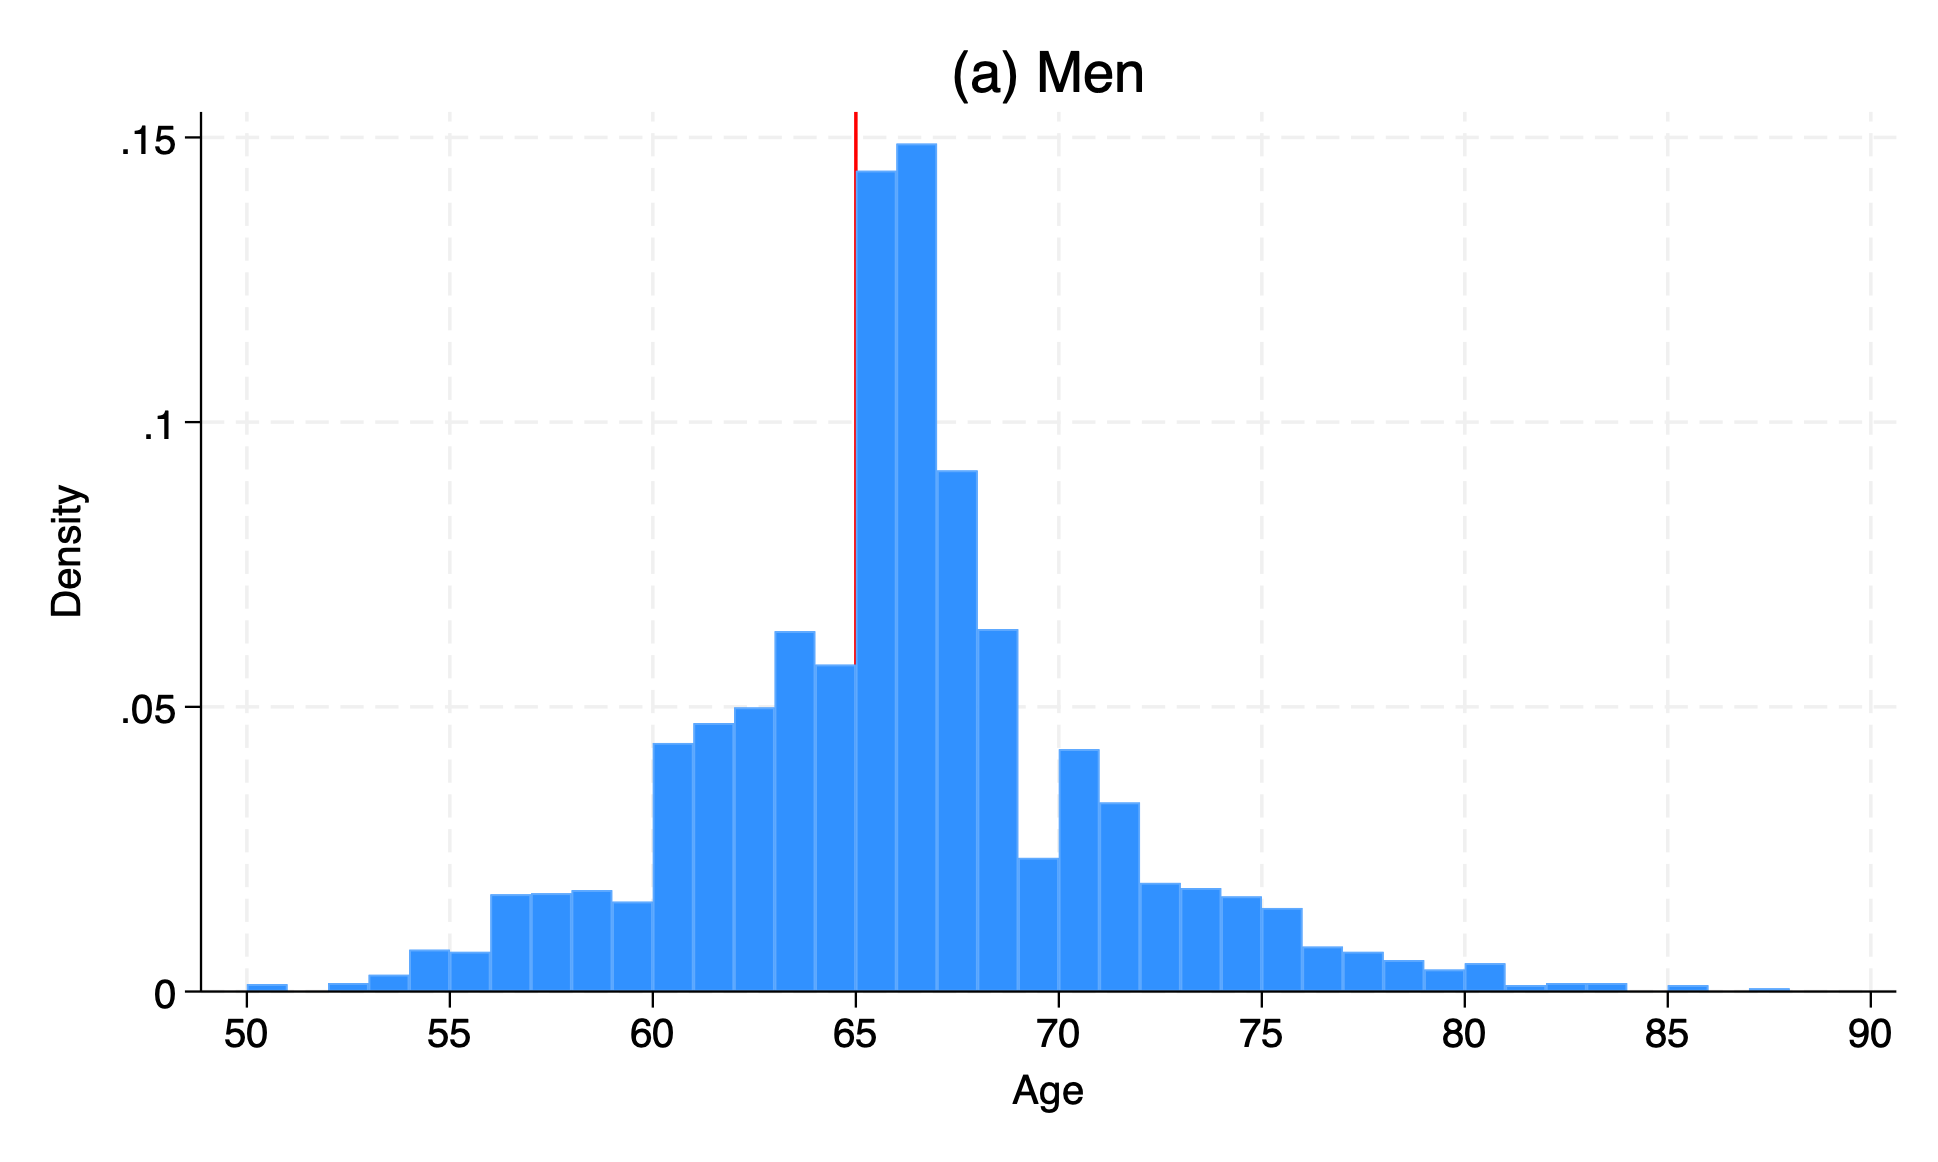
\includegraphics[width=1.1\textwidth]{male.png} \\[0.1cm] % Adds space between images
    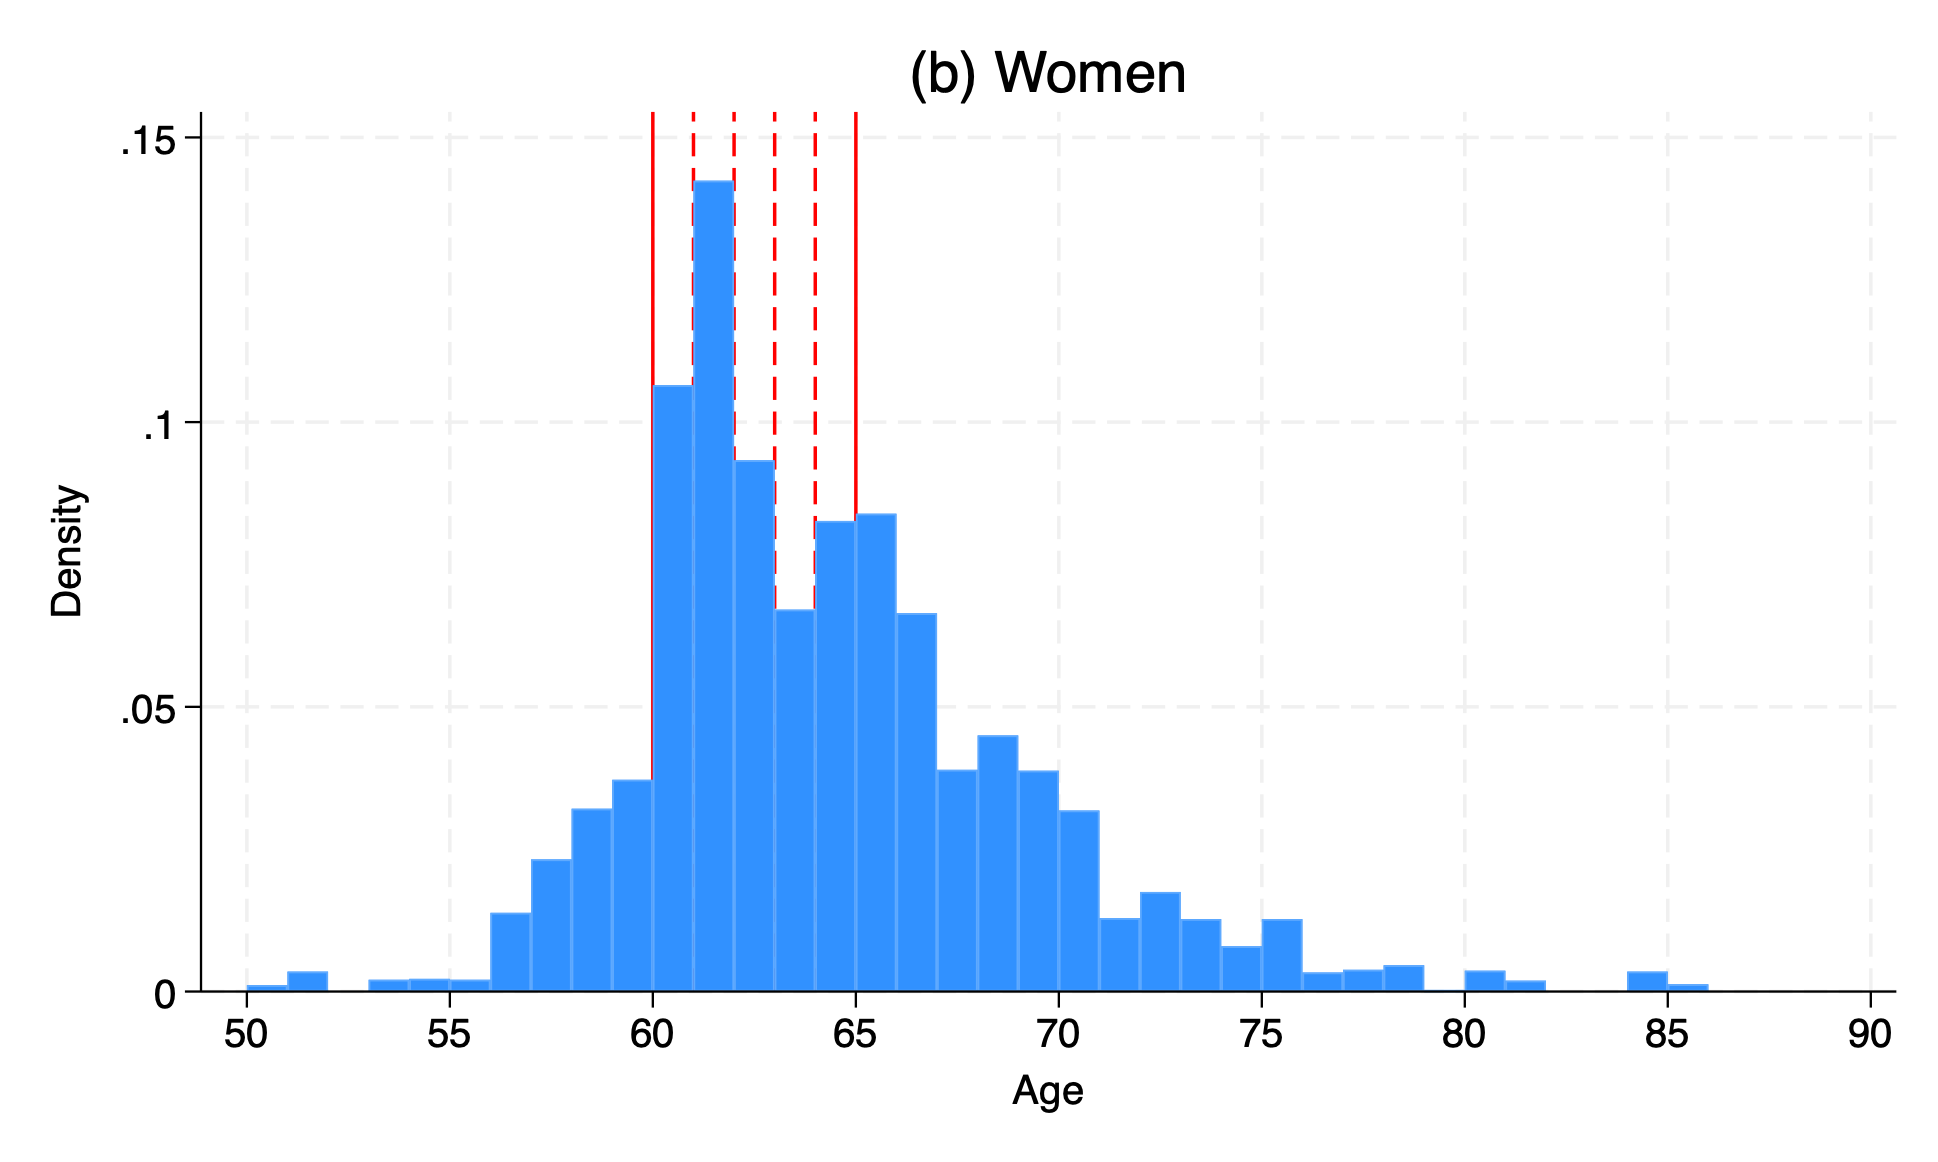
\includegraphics[width=1.1\textwidth]{female.png}

    % Right Column - Bullet Points
    \column{0.55\textwidth}
    \begin{itemize}
    \scriptsize
      \item<1->  To handle this type of endogeneity, we can use an \begingroup\color{Blue}Instrumental Variable (IV) \endgroup approach
      
       \item<2-> A variable ($D_{ijt}$) that impacts mental health only \begingroup\color{Blue}indirectly \endgroup by influencing the retirement decision ($RET_{ijt}$)
      
      \item<3->  \begingroup\color{Blue}\textbf{Statutory Pension Age (SPA)} \endgroup as an instrument variable \begingroup\color{lightgray}(Carrino et al., 2020)\endgroup
      \item<4-> \begingroup\color{Blue}Men \endgroup maintained a state pension age of 65 from 2002 to 2019
      \item<5-> \begingroup\color{Blue}Women\endgroup’s SPA started at 60 in 2002 and gradually increased from April 2010, reaching 65 by November 2018 to equalise with men. 

       \item<6->  Our analysis counts for these \begingroup\color{Blue}alterations  \endgroup in the eligibility rules for women
    \end{itemize}

\end{columns}

\end{frame}

\begin{frame}{Intensity of economic crisis}
 \framesubtitle{Regions severely hit by economic crises}
\footnotesize
\begin{figure}
    \centering
    \tiny
    \caption*{\scriptsize \begingroup\color{Blue}Figure: \endgroup 
Percentage point increases in unemployment rates pre- vs post-economic crisis }
    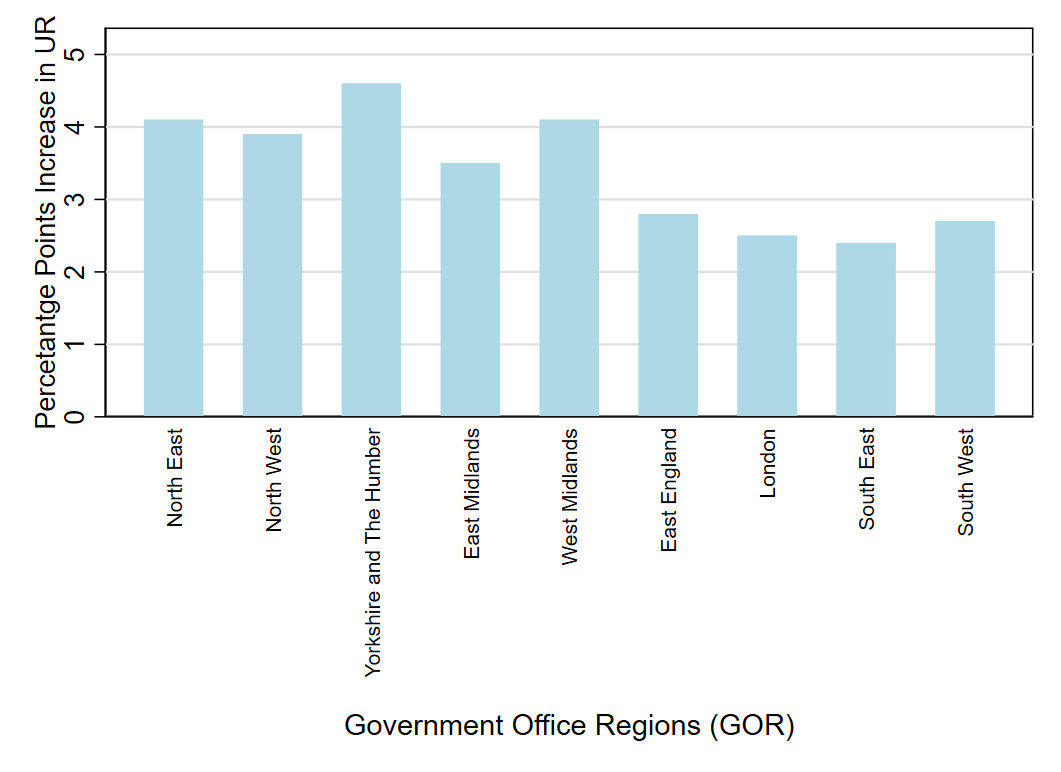
\includegraphics[width=0.8\linewidth]{UnempPP.png}
    \label{fig1}
    \vspace*{-0.5cm}
     
\end{figure}
\vspace*{-0.75cm}
\begin{block}
\scriptsize
\centering
Living in a \begingroup\color{Blue} severely \endgroup  hit area if the region experiences an increase in the unemployment rate to be in the \begingroup\color{Blue}top 75 percentile \endgroup \begingroup\color{lightgray}(ONS)\endgroup
\end{block}


\end{frame}

\begin{frame}{Empirical Strategies (II): IV-FE}
\footnotesize

We therefore estimate Equation 2 using \begingroup\color{Blue}IV-FE estimators\endgroup:

\begin{equation}
\label{eq2}
\begin{aligned}
  Y_{ijt} &= \alpha + \delta_{D} D_{itj} + \delta_{RH} D_{itj}HIT_{tj} + \delta_{HIT} HIT_{tj} \\
  &\quad + \gamma_X X_{ijt} + \omega_w W_{jt} + Wave_{t} + Region_j + d_i + e_{ijt}
\end{aligned}
\end{equation}
\vspace{0.25cm}
\begin{itemize}
\scriptsize
\item  Two \begingroup\color{Blue}instruments \endgroup for retirement: 

\vspace{0.25cm}

\begin{enumerate}
\scriptsize
    \item<2-> The \begingroup\color{Blue}statutory retirement eligibility age \endgroup dummy ($D_{ijt}$)

    \vspace{0.25cm}
    
    \item<3-> An interaction term that combines the \begingroup\color{Blue}economic crisis region indicator ($HIT_{jt}$) \endgroup with the statutory retirement age dummy ($D_{ijt}$)
\end{enumerate}

\vspace{0.5cm}

\item<4-> $\delta_{RH}$ is our \begingroup\color{Blue}parameter of interest \endgroup in capturing the effect of retirement in a region severely hit by the economic crisis
\end{itemize}
\end{frame}





\section{Results}



\begin{frame}{Descriptive Statistics}

\begin{table}[h]
\centering
\label{tab1}
\resizebox{0.85\textwidth}{!}{%
\begin{tabular}{cccccc}
\toprule
\multirow{2}{*}{\textbf{Variables}} & \multicolumn{2}{c}{\textbf{Employed}} & \multicolumn{2}{c}{\textbf{Retired}} & \multirow{2}{*}{\textbf{Test for Mean Differences}} \\ 
 & \textit{Mean} & \textit{SD} & \textit{Mean} & \textit{SD} &  \\ \hline
\multicolumn{6}{l}{\textbf{a) Socio-demographics}} \\\hline
\textit{Female} & 0.461 & 0.499 & 0.503 & 0.500 &  \\
\textit{Age} & 61.17 & 5.502 & 68.49 & 5.986 & *** \\
\textit{Married/Cohabitee} & 0.770 & 0.421 & 0.731 & 0.443 & *** \\
\textit{Number of people in the household (adults+children)} & 2.217 & 0.841 & 1.948 & 0.678 & *** \\
\textit{Tenure (home owner outright)} & 0.578 & 0.494 & 0.818 & 0.386 & *** \\
\multicolumn{6}{l}{Education} \\
\multicolumn{1}{l}{\textit{never went or not yet finished}} & 0.011 & 0.105 & 0.008 & 0.092 &  \\
\textit{went to school until 14 or below} & 0.016 & 0.126 & 0.030 & 0.171 & *** \\
\textit{O levels} & 0.488 & 0.500 & 0.506 & 0.500 &  \\
\textit{A levels} & 0.118 & 0.323 & 0.105 & 0.306 &  \\
\textit{Higher education below degree} & 0.148 & 0.355 & 0.149 & 0.356 & ** \\
\textit{Degree} & 0.219 & 0.413 & 0.202 & 0.401 &  \\\hline
\multicolumn{6}{l}{\textbf{b) Regional Characteristics}} \\\hline
\multicolumn{6}{l}{Population Density for Postcode Sectors} \\
\textit{First quintile (least dense)} & 0.193 & 0.394 & 0.197 & 0.398 &  \\
\textit{Second quintile} & 0.242 & 0.428 & 0.246 & 0.431 &  \\
\textit{Third quintile} & 0.213 & 0.410 & 0.230 & 0.421 & ** \\
\textit{Fourth quintile} & 0.195 & 0.396 & 0.183 & 0.386 &  \\
\textit{Fifth quintile (most dense)} & 0.158 & 0.364 & 0.144 & 0.351 & *** \\
\multicolumn{6}{l}{Index of Multiple Deprivation Score} \\
\textit{First quintile (least deprived)} & 0.263 & 0.440 & 0.271 & 0.445 &  \\
\textit{Second quintile} & 0.263 & 0.440 & 0.257 & 0.437 &  \\
\textit{Third quintile} & 0.207 & 0.405 & 0.200 & 0.400 & ** \\
\textit{Fourth quintile} & 0.158 & 0.365 & 0.172 & 0.377 &  \\
\textit{Fifth quintile (most deprived)} & 0.109 & 0.312 & 0.099 & 0.300 & ** \\\hline
\multicolumn{6}{l}{\textbf{c) Pension characteristics and financial variables}} \\\hline
\textit{Aged equal or above the State Pension Age (SPA)} & 0.372 & 0.483 & 0.887 & 0.317 & *** \\
\textit{Member of private pension scheme} & 0.809 & 0.393 & 0.799 & 0.401 &  \\
\textit{\begin{tabular}[c]{@{}c@{}}Total state pension wealth \\ (£ per week)\end{tabular}} & 62.49 & 89.74 & 173.9 & 97.56 & *** \\
\textit{Whether under financial strain} & 0.044 & 0.206 & 0.027 & 0.165 & *** \\\hline
\multicolumn{1}{l}{\textbf{d)Health related-behaviours}} &  &  &  &  &  \\\hline
\textit{Never smoked} & 0.354 & 0.478 & 0.353 & 0.478 &  \\
\textit{Engages with vigorous physical activity (at least once per week)} & 0.385 & 0.487 & 0.344 & 0.475 & *** \\
\textit{Private health insurance} & 0.191 & 0.393 & 0.096 & 0.295 & *** \\
\multicolumn{1}{l}{Observations} & \multicolumn{2}{c}{8,900} & \multicolumn{2}{c}{6,588} & \\\hline
\end{tabular}%
}
\end{table}

\end{frame}


\begin{frame}{Results (I): Retirement and Mental Health}

     \footnotesize
\begin{figure}
    \centering
    \caption*{\footnotesize \begingroup\color{Blue} Figure: \endgroup \scriptsize  Results of the relationship between health and retirement (all sample): short-term analyses (2004-2013)}
    
\includegraphics[width=0.9\linewidth]{Figure2.png}
    \label{fig1}
    
\end{figure}

\end{frame}

\begin{frame}{Results (I): Heterogenous Analyses}
\framesubtitle{Mental Health}
    \begin{table}[h]
\centering

\label{tab2}
\resizebox{\textwidth}{!}{%
\begin{tabular}{@{}ccccccccc@{}}
\toprule
\multirow{2}{*}{\textbf{Outcome variables}} & \multicolumn{2}{c}{\textbf{\begin{tabular}[c]{@{}c@{}}(a) \\ All sample\end{tabular}}} & \multicolumn{2}{c}{\textbf{\begin{tabular}[c]{@{}c@{}}(b)\\ Women\end{tabular}}} & \multicolumn{2}{c}{\textbf{\begin{tabular}[c]{@{}c@{}}(c)\\ Blue-collar\end{tabular}}} & \multicolumn{2}{c}{\textbf{\begin{tabular}[c]{@{}c@{}}(d) \\ Above unemployment average\end{tabular}}} \\ \cmidrule(l){2-9} 
 & \textbf{FE} & \textbf{IV-FE} & \textbf{FE} & \textbf{IV-FE} & \textbf{FE} & \textbf{IV-FE} & \textbf{FE} & \textbf{IV-FE} \\ \hline
\multicolumn{9}{l}{\textbf{(1) Depression Symptoms {[}0-8{]}}} \\ \hline
\multicolumn{1}{l}{Retired} & \begin{tabular}[c]{@{}c@{}}-0.035\\ (0.046)\end{tabular} & \begin{tabular}[c]{@{}c@{}}-0.160\\ (0.381)\end{tabular} & \begin{tabular}[c]{@{}c@{}}-0.040\\ (0.070)\end{tabular} & \begin{tabular}[c]{@{}c@{}}-0.689\\ (0.059)\end{tabular} & \begin{tabular}[c]{@{}c@{}}-0.021\\ (0.070)\end{tabular} & \begin{tabular}[c]{@{}c@{}}-0.036\\ (0.459)\end{tabular} & \begin{tabular}[c]{@{}c@{}}-0.041\\ (0.061)\end{tabular} & \begin{tabular}[c]{@{}c@{}}0.755\\ (0.624)\end{tabular} \\
\multicolumn{1}{r}{First stage} &  & \begin{tabular}[c]{@{}c@{}}0.151***\\ (0.017)\end{tabular} &  & \begin{tabular}[c]{@{}c@{}}0.133***\\ (0.020)\end{tabular} &  & \begin{tabular}[c]{@{}c@{}}0.198***\\ (0.025)\end{tabular} &  & \begin{tabular}[c]{@{}c@{}}0.120***\\ (0.021)\end{tabular} \\
\multicolumn{1}{r}{Weak identification: F-test of excluded instruments} &  & 103.77*** &  & 57.94*** &  & 99.63*** &  & 42.27*** \\\hline
\multicolumn{9}{l}{\textbf{(2) Newly diagnosed psychiatric condition±}} \\\hline
\multicolumn{1}{l}{Retired} & \begin{tabular}[c]{@{}c@{}}0.002\\ (0.005)\end{tabular} & \begin{tabular}[c]{@{}c@{}}-0.026\\ (0.041)\end{tabular} & \begin{tabular}[c]{@{}c@{}}-0.002\\ (0.008)\end{tabular} & \begin{tabular}[c]{@{}c@{}}-0.050\\ (0.065)\end{tabular} & \begin{tabular}[c]{@{}c@{}}-0.004\\ (0.006)\end{tabular} & \begin{tabular}[c]{@{}c@{}}-0.012\\ (0.046)\end{tabular} & \begin{tabular}[c]{@{}c@{}}0.011*\\ (0.006)\end{tabular} & \begin{tabular}[c]{@{}c@{}}0.042\\ (0.05)\end{tabular} \\
\multicolumn{1}{r}{First stage} &  & \begin{tabular}[c]{@{}c@{}}0.151***\\ (0.017)\end{tabular} &  & \begin{tabular}[c]{@{}c@{}}0.133***\\ (0.020)\end{tabular} &  & \begin{tabular}[c]{@{}c@{}}0.198***\\ (0.025)\end{tabular} & \textbf{} & \begin{tabular}[c]{@{}c@{}}0.120***\\ (0.021)\end{tabular} \\
\multicolumn{1}{r}{Weak identification: F-test of excluded instruments} &  & 103.85*** &  & 57.94*** &  & 99.63*** & \textbf{} & 42.27*** \\
\textit{Control variables} & \textit{\checkmark} & \textit{\checkmark} & \textit{\checkmark} & \textit{\checkmark} & \textit{\checkmark} & \textit{\checkmark} & \textit{\checkmark} & \textit{\checkmark} \\
\textit{Region and Time FE} & \textit{\checkmark} & \textit{\checkmark} & \textit{\checkmark} & \textit{\checkmark} & \textit{\checkmark} & \textit{\checkmark} & \textit{\checkmark} & \textit{\checkmark} \\
\textit{Observations} & \multicolumn{2}{c}{10,273} & \multicolumn{2}{c}{5,480} & \multicolumn{2}{c}{5,100} & \multicolumn{2}{c}{6,531} \\
\textit{Number IDs} & \multicolumn{2}{c}{2,638} & \multicolumn{2}{c}{1,409} & \multicolumn{2}{c}{1,513} & \multicolumn{2}{c}{2,298} \\ \bottomrule
\end{tabular}%
}
\end{table}
\end{frame}



\begin{frame}{Results (I): Heterogenous Analyses}
\framesubtitle{Well-being}
    \begin{table}[h]
\centering

\label{tab21}
\resizebox{\textwidth}{!}{%
\begin{tabular}{ccccccccc}
\toprule
\multirow{2}{*}{\textbf{Outcome variables}} & \multicolumn{2}{c}{\textbf{\begin{tabular}[c]{@{}c@{}}(a) \\ All sample\end{tabular}}} & \multicolumn{2}{c}{\textbf{\begin{tabular}[c]{@{}c@{}}(b)\\ Women\end{tabular}}} & \multicolumn{2}{c}{\textbf{\begin{tabular}[c]{@{}c@{}}(c)\\ Blue-collar\end{tabular}}} & \multicolumn{2}{c}{\textbf{\begin{tabular}[c]{@{}c@{}}(d) \\ Above unemployment average\end{tabular}}} \\
 & \textbf{FE} & \textbf{IV-FE} & \textbf{FE} & \textbf{IV-FE} & \textbf{FE} & \textbf{IV-FE} & \textbf{FE} & \textbf{IV-FE} \\\hline
\multicolumn{9}{l}{\textbf{(3) Feeling lonely±}} \\\hline
\multicolumn{1}{l}{Retired} & \begin{tabular}[c]{@{}c@{}}0.002\\ (0.009)\end{tabular} & \begin{tabular}[c]{@{}c@{}}0.148**\\ (0.068)\end{tabular} & \begin{tabular}[c]{@{}c@{}}0.018\\ (0.013)\end{tabular} & \begin{tabular}[c]{@{}c@{}}0.286***\\ (0.096)\end{tabular} & \begin{tabular}[c]{@{}c@{}}0.015\\ (0.015)\end{tabular} & \begin{tabular}[c]{@{}c@{}}0.140*\\ (0.081)\end{tabular} & \begin{tabular}[c]{@{}c@{}}-0.010\\ (0.014)\end{tabular} & \begin{tabular}[c]{@{}c@{}}0.330**\\ (0.141)\end{tabular} \\
\multicolumn{1}{r}{First stage} & \textbf{} & \begin{tabular}[c]{@{}c@{}}0.158***\\ (0.018)\end{tabular} & \textbf{} & \begin{tabular}[c]{@{}c@{}}0.145*\\ (0.022)\end{tabular} & \textbf{} & \begin{tabular}[c]{@{}c@{}}0.200***\\ (0.000)\end{tabular} & \textbf{} & \begin{tabular}[c]{@{}c@{}}0.125***\\ (0.0234)\end{tabular} \\
\multicolumn{1}{r}{Weak identification: F-test of excluded instruments} & \textbf{} & 97.17*** & \textbf{} & 58.52*** & \textbf{} & 84.75*** & \textbf{} & 38.83*** \\\hline
\multicolumn{9}{l}{\textbf{(4) Life satisfaction±}} \\\hline
\multicolumn{1}{l}{Retired} & \begin{tabular}[c]{@{}c@{}}0.024\\ (0.015)\end{tabular} & \begin{tabular}[c]{@{}c@{}}0.063\\ (0.110)\end{tabular} & \begin{tabular}[c]{@{}c@{}}0.031\\ (0.019)\end{tabular} & \begin{tabular}[c]{@{}c@{}}0.083\\ (0.154)\end{tabular} & \begin{tabular}[c]{@{}c@{}}0.022\\ (0.022)\end{tabular} & \begin{tabular}[c]{@{}c@{}}-0.023\\ (0.131)\end{tabular} & \begin{tabular}[c]{@{}c@{}}0.039**\\ (0.019)\end{tabular} & \begin{tabular}[c]{@{}c@{}}-0.143\\ (0.193)\end{tabular} \\
\multicolumn{1}{r}{First stage} &  & \begin{tabular}[c]{@{}c@{}}48.08***\\ (0.000)\end{tabular} &  & \begin{tabular}[c]{@{}c@{}}0.145***\\ (0.000)\end{tabular} &  & \begin{tabular}[c]{@{}c@{}}0.198***\\ (0.000)\end{tabular} &  & \begin{tabular}[c]{@{}c@{}}0.124***\\ (0.000)\end{tabular} \\
\multicolumn{1}{r}{Weak identification: F-test of excluded instruments} &  & 101.52*** &  & 60.05*** &  & 86.57*** &  & 38.17*** \\
\textit{Control variables} & \textit{\checkmark} & \textit{\checkmark} & \textit{\checkmark} & \textit{\checkmark} & \textit{\checkmark} & \textit{\checkmark} & \textit{\checkmark} & \textit{\checkmark} \\
\textit{Region and Time FE} & \textit{\checkmark} & \textit{\checkmark} & \textit{\checkmark} & \textit{\checkmark} & \textit{\checkmark} & \textit{\checkmark} & \textit{\checkmark} & \textit{\checkmark} \\
\textit{Observations} & \multicolumn{2}{c}{10,273} & \multicolumn{2}{c}{5,480} & \multicolumn{2}{c}{5,100} & \multicolumn{2}{c}{6,531} \\
\textit{Number IDs} & \multicolumn{2}{c}{2,638} & \multicolumn{2}{c}{1,409} & \multicolumn{2}{c}{1,513} & \multicolumn{2}{c}{2,298} \\\hline
\end{tabular}%
}
\end{table}
\end{frame}

\begin{frame}{Results (II): Retirement, Economic Shock and Mental Health}
    \framesubtitle{Short-term analyses (2004-2013): Mental Health}

    \begin{table}[h]
\centering

\label{tab3}
\resizebox{\textwidth}{!}{%
\begin{tabular}{@{}lccccccccc@{}}
\toprule
\multicolumn{1}{c}{\multirow{2}{*}{\textbf{Outcome variables}}} & \multicolumn{3}{c}{\textbf{\begin{tabular}[c]{@{}c@{}}(a)\\ All sample\end{tabular}}} & \multicolumn{3}{c}{\textbf{\begin{tabular}[c]{@{}c@{}}(b)\\ Men\end{tabular}}} & \multicolumn{3}{c}{\textbf{\begin{tabular}[c]{@{}c@{}}(c)\\ Women\end{tabular}}} \\ \cmidrule(l){2-10} 
\multicolumn{1}{c}{} & \textbf{All} & \textbf{White-collar} & \textbf{Blue-collar} & \textbf{All Men} & \textbf{White-collar} & \textbf{Blue-collar} & \textbf{All Women} & \textbf{White-collar} & \textbf{Blue-collar} \\ \hline
\multicolumn{10}{l}{\textbf{(1) Depression Symptoms {[}0-8{]}}} \\\hline
Retired & \begin{tabular}[c]{@{}c@{}}-0.259\\ (0.392)\end{tabular} & \begin{tabular}[c]{@{}c@{}}-0.483\\ (0.690)\end{tabular} & \begin{tabular}[c]{@{}c@{}}-0.126\\ (0.486)\end{tabular} & \begin{tabular}[c]{@{}c@{}}0.605\\ (0.459)\end{tabular} & \begin{tabular}[c]{@{}c@{}}0.677\\ (0.737)\end{tabular} & \begin{tabular}[c]{@{}c@{}}0.651\\ (0.652)\end{tabular} & \begin{tabular}[c]{@{}c@{}}-0.726\\ (0.590)\end{tabular} & \begin{tabular}[c]{@{}c@{}}-2.042\\ (1.466)\end{tabular} & \begin{tabular}[c]{@{}c@{}}-0.345\\ (0.636)\end{tabular} \\
\textit{Retired x hit by high unemployment} & \textit{\begin{tabular}[c]{@{}c@{}}0.286\\ (0.218)\end{tabular}} & \textit{\begin{tabular}[c]{@{}c@{}}0.428\\ (0.335)\end{tabular}} & \textit{\begin{tabular}[c]{@{}c@{}}0.076\\ (0.295)\end{tabular}} & \textit{\begin{tabular}[c]{@{}c@{}}-0.053\\ (0.270)\end{tabular}} & \textit{\begin{tabular}[c]{@{}c@{}}0.336\\ (0.375)\end{tabular}} & \textit{\begin{tabular}[c]{@{}c@{}}-0.609\\ (0.433)\end{tabular}} & \textit{\begin{tabular}[c]{@{}c@{}}0.498\\ (0.328)\end{tabular}} & \textit{\begin{tabular}[c]{@{}c@{}}0.039\\ (0.725)\end{tabular}} & \textit{\begin{tabular}[c]{@{}c@{}}0.550\\ (0.375)\end{tabular}} \\
Hit by high unemployment & \begin{tabular}[c]{@{}c@{}}-0.183**\\ (0.091)\end{tabular} & \begin{tabular}[c]{@{}c@{}}-0.289**\\ (0.132)\end{tabular} & \begin{tabular}[c]{@{}c@{}}-0.012\\ (0.132)\end{tabular} & \begin{tabular}[c]{@{}c@{}}-0.118\\ (0.111)\end{tabular} & \begin{tabular}[c]{@{}c@{}}-0.270*\\ (0.147)\end{tabular} & \begin{tabular}[c]{@{}c@{}}0.166\\ (0.187)\end{tabular} & \begin{tabular}[c]{@{}c@{}}-0.207\\ (0.147)\end{tabular} & \begin{tabular}[c]{@{}c@{}}-0.062\\ (0.301)\end{tabular} & \begin{tabular}[c]{@{}c@{}}-0.171\\ (0.178)\end{tabular} \\
\multicolumn{1}{r}{Weak identification: F-test (Retired)} & 53.30*** & 16.17*** & 51.78*** & 33.87*** & 10.40*** & 24.96 *** & 29.42*** & 5.57*** & 29.50*** \\
\multicolumn{1}{r}{\begin{tabular}[c]{@{}r@{}}Weak identification: \\ F-test (Retired x hit high unemp.)\end{tabular}} & 260.99*** & 127.44*** & 195.94*** & 157.69*** & \multicolumn{1}{l}{79.07***} & 73.51*** & 162.31*** & 44.44*** & 121.16*** \\\hline
\multicolumn{10}{l}{\textbf{(2) Newly diagnosed psychiatric condition±}} \\\hline
Retired & \begin{tabular}[c]{@{}c@{}}-0.012\\ (0.043)\end{tabular} & \begin{tabular}[c]{@{}c@{}}0.001\\ (0.080)\end{tabular} & \begin{tabular}[c]{@{}c@{}}-0.004\\ (0.051)\end{tabular} & \begin{tabular}[c]{@{}c@{}}0.046\\ (0.050)\end{tabular} & \begin{tabular}[c]{@{}c@{}}-0.017\\ (0.084)\end{tabular} & \begin{tabular}[c]{@{}c@{}}0.135\\ (0.073)\end{tabular} & \begin{tabular}[c]{@{}c@{}}-.046\\ (0.066)\end{tabular} & \begin{tabular}[c]{@{}c@{}}0.057\\ (0.154)\end{tabular} & \begin{tabular}[c]{@{}c@{}}-0.087\\ (0.068)\end{tabular} \\
\textit{Retired x hit by high unemployment} & \textit{\begin{tabular}[c]{@{}c@{}}-0.049**\\ (0.023)\end{tabular}} & \textit{\begin{tabular}[c]{@{}c@{}}-0.062*\\ (0.037)\end{tabular}} & \textit{\begin{tabular}[c]{@{}c@{}}-0.030\\ (0.030)\end{tabular}} & \textit{\begin{tabular}[c]{@{}c@{}}-0.051*\\ (0.028)\end{tabular}} & \textit{\begin{tabular}[c]{@{}c@{}}-0.055\\ (0.041)\end{tabular}} & \textit{\begin{tabular}[c]{@{}c@{}}-0.058\\ (0.043)\end{tabular}} & \textit{\begin{tabular}[c]{@{}c@{}}-0.044\\ (0.035)\end{tabular}} & \textit{\begin{tabular}[c]{@{}c@{}}-0.073\\ (0.072)\end{tabular}} & \textit{\begin{tabular}[c]{@{}c@{}}-0.003\\ (0.041)\end{tabular}} \\
Hit by high unemployment & \begin{tabular}[c]{@{}c@{}}0.023**\\ (0.010)\end{tabular} & \begin{tabular}[c]{@{}c@{}}0.029*\\ (0.015)\end{tabular} & \begin{tabular}[c]{@{}c@{}}0.017\\ (0.013)\end{tabular} & \begin{tabular}[c]{@{}c@{}}0.022\\ (0.011)\end{tabular} & \begin{tabular}[c]{@{}c@{}}0.021\\ (0.016)\end{tabular} & \begin{tabular}[c]{@{}c@{}}0.032*\\ (0.019)\end{tabular} & \begin{tabular}[c]{@{}c@{}}0.023\\ (0.015)\end{tabular} & \begin{tabular}[c]{@{}c@{}}0.042\\ (0.030)\end{tabular} & \begin{tabular}[c]{@{}c@{}}0.004\\ (0.017)\end{tabular} \\
\multicolumn{1}{r}{Weak identification: F-test (Retired)} & 53.30*** & 13.87*** & 43.13*** & 25.73*** & 8.32*** & 17.74*** & 27.44*** & 7.05*** & 19.92*** \\
\multicolumn{1}{r}{\begin{tabular}[c]{@{}r@{}}Weak identification:\\  F-test (Retired x hit by high unemp.)\end{tabular}} & 260.99*** & 94.43*** & 165.60*** & 111.20*** & 56.95*** & 51.32*** & 157.22*** & 41.92*** & 132.14*** \\
\multicolumn{1}{c}{\textit{Control variables}} & \textit{\checkmark} & \textit{\checkmark} & \textit{\checkmark} & \textit{\checkmark} & \textit{\checkmark} & \textit{\checkmark} & \textit{\checkmark} & \textit{\checkmark} & \textit{\checkmark} \\
\multicolumn{1}{c}{\textit{Region and Time FE}} & \textit{\checkmark} & \textit{\checkmark} & \textit{\checkmark} & \textit{\checkmark} & \textit{\checkmark} & \textit{\checkmark} & \textit{\checkmark} & \textit{\checkmark} & \textit{\checkmark} \\
\multicolumn{1}{c}{\textit{Observations}} & 10,273 & 5,173 & 5,100 & 4,793 & 2,829 & 1,964 & 5,480 & 2,153 & 3,136 \\
\multicolumn{1}{c}{\textit{Number IDs}} & 2,638 & 1,333 & 1,513 & 1,229 & 715 & 616 & 1,409 & 594 & 897 \\ \bottomrule
\end{tabular}%
}
\end{table}
\end{frame}


\begin{frame}{Results (II): Retirement, Economic Shock and Mental Health}
    \framesubtitle{Short-term analyses (2004-2013): Well-being}

\begin{table}[h]
\centering
\label{tab31}
\resizebox{\textwidth}{!}{%
\begin{tabular}{@{}lccccccccc@{}}
\toprule
\multicolumn{1}{c}{\multirow{2}{*}{\textbf{Outcome variables}}} & \multicolumn{3}{c}{\textbf{\begin{tabular}[c]{@{}c@{}}(a)\\ All sample\end{tabular}}} & \multicolumn{3}{c}{\textbf{\begin{tabular}[c]{@{}c@{}}(b)\\ Men\end{tabular}}} & \multicolumn{3}{c}{\textbf{\begin{tabular}[c]{@{}c@{}}(c)\\ Women\end{tabular}}} \\
\multicolumn{1}{c}{} & \textbf{All} & \textbf{White-collar} & \textbf{Blue-collar} & \textbf{All Men} & \textbf{White-collar} & \textbf{Blue-collar} & \textbf{All Women} & \textbf{White-collar} & \textbf{Blue-collar} \\\hline
\multicolumn{10}{l}{\textbf{(3) Feeling lonely±}} \\\hline
Retired & \begin{tabular}[c]{@{}c@{}}0.147**\\ (0.070)\end{tabular} & \begin{tabular}[c]{@{}c@{}}0.163\\ (0.120)\end{tabular} & \begin{tabular}[c]{@{}c@{}}0.148*\\ (0.084)\end{tabular} & \begin{tabular}[c]{@{}c@{}}-0.115\\ (0.113)\end{tabular} & \begin{tabular}[c]{@{}c@{}}-.0176\\ (0.178)\end{tabular} & \begin{tabular}[c]{@{}c@{}}0.024\\ (0.148)\end{tabular} & \begin{tabular}[c]{@{}c@{}}0.285***\\ (0.096)\end{tabular} & \begin{tabular}[c]{@{}c@{}}0.489***\\ (0.250)\end{tabular} & \begin{tabular}[c]{@{}c@{}}0.184\\ (0.104)\end{tabular} \\
Retired x hit by high unemployment & \begin{tabular}[c]{@{}c@{}}0.007\\ (0.044)\end{tabular} & \begin{tabular}[c]{@{}c@{}}0.052\\ (0.069)\end{tabular} & \begin{tabular}[c]{@{}c@{}}-0.014\\ (0.060)\end{tabular} & \begin{tabular}[c]{@{}c@{}}0.066\\ (0.071)\end{tabular} & \begin{tabular}[c]{@{}c@{}}0.014\\ (0.093)\end{tabular} & \begin{tabular}[c]{@{}c@{}}0.115\\ (0.121)\end{tabular} & \begin{tabular}[c]{@{}c@{}}0.008\\ (0.064)\end{tabular} & \begin{tabular}[c]{@{}c@{}}0.175\\ (0.147)\end{tabular} & \begin{tabular}[c]{@{}c@{}}-0.054\\ (0.075)\end{tabular} \\
Hit by high unemployment & \begin{tabular}[c]{@{}c@{}}0.009\\ (0.019)\end{tabular} & \begin{tabular}[c]{@{}c@{}}-0.010\\ (0.027)\end{tabular} & \begin{tabular}[c]{@{}c@{}}0.018\\ (0.028)\end{tabular} & \begin{tabular}[c]{@{}c@{}}-0.001\\ (0.026)\end{tabular} & \begin{tabular}[c]{@{}c@{}}-0.006\\ (0,033)\end{tabular} & \begin{tabular}[c]{@{}c@{}}0.015\\ (0.048)\end{tabular} & \begin{tabular}[c]{@{}c@{}}-0.002\\ (0.029)\end{tabular} & \begin{tabular}[c]{@{}c@{}}-.070\\ (0.060)\end{tabular} & \begin{tabular}[c]{@{}c@{}}.017\\ (0.037)\end{tabular} \\
\multicolumn{1}{r}{Weak identification: F-test (Retired)} & 58.24*** & 18.51*** & 20.29*** & 27.69*** & 11.07*** & 17.72*** & 29.50*** & 7.05*** & 26.89*** \\
\multicolumn{1}{r}{\begin{tabular}[c]{@{}r@{}}Weak identification: \\ F-test (Retired x hit high unemp.)\end{tabular}} & 292.24*** & 124.76*** & 129.10*** & 134.62*** & 75.49*** & 53.96*** & 144.34*** & 41.92*** & 104.94*** \\\hline
\multicolumn{10}{l}{\textbf{(4) Life satisfaction±}} \\\hline
Retired & \begin{tabular}[c]{@{}c@{}}0.061\\ (0.113)\end{tabular} & \begin{tabular}[c]{@{}c@{}}0.127\\ (0.198)\end{tabular} & \begin{tabular}[c]{@{}c@{}}-0.016\\ (0.137)\end{tabular} & \begin{tabular}[c]{@{}c@{}}-0.021\\ (0.173)\end{tabular} & \begin{tabular}[c]{@{}c@{}}-0.154\\ (0.288)\end{tabular} & \begin{tabular}[c]{@{}c@{}}0.143\\ (0.232)\end{tabular} & \begin{tabular}[c]{@{}c@{}}0.088\\ (.155)\end{tabular} & \begin{tabular}[c]{@{}c@{}}0.420\\ (0.324)\end{tabular} & \begin{tabular}[c]{@{}c@{}}-0.149\\ (0.175)\end{tabular} \\
\textit{Retired x hit by high unemployment} & \begin{tabular}[c]{@{}c@{}}-0.010\\ (0.064)\end{tabular} & \begin{tabular}[c]{@{}c@{}}0.093\\ (0.099)\end{tabular} & \begin{tabular}[c]{@{}c@{}}-.059\\ (0.094)\end{tabular} & \begin{tabular}[c]{@{}c@{}}0.034\\ (0.094)\end{tabular} & \begin{tabular}[c]{@{}c@{}}0.088\\ (0.124)\end{tabular} & \begin{tabular}[c]{@{}c@{}}-0.063\\ (0.141)\end{tabular} & \begin{tabular}[c]{@{}c@{}}-0.108\\ (0.091)\end{tabular} & \begin{tabular}[c]{@{}c@{}}0.073\\ (0.181)\end{tabular} & \begin{tabular}[c]{@{}c@{}}-0.149\\ (0.115)\end{tabular} \\
Hit by high unemployment & \begin{tabular}[c]{@{}c@{}}-0.015\\ (0.029)\end{tabular} & \begin{tabular}[c]{@{}c@{}}-0.034\\ (0.027)\end{tabular} & \begin{tabular}[c]{@{}c@{}}-0.010\\ (0.047)\end{tabular} & \begin{tabular}[c]{@{}c@{}}-0.053\\ (0.040)\end{tabular} & \begin{tabular}[c]{@{}c@{}}-0.065\\ (0.049)\end{tabular} & \begin{tabular}[c]{@{}c@{}}-0.035\\ (0.079)\end{tabular} & \begin{tabular}[c]{@{}c@{}}0.043\\ (0.044)\end{tabular} & \begin{tabular}[c]{@{}c@{}}0.001\\ (0.079)\end{tabular} & \begin{tabular}[c]{@{}c@{}}0.042\\ (0.057)\end{tabular} \\
\multicolumn{1}{r}{Weak identification: F-test (Retired)} & 61.37*** & 20.29*** & 44.72*** & 30.33*** & 11.25*** & 20.40*** & 30.31*** & 8.35*** & 25.95*** \\
\multicolumn{1}{r}{\begin{tabular}[c]{@{}r@{}}Weak identification: \\ F-test (Retired x hit high unemp.)\end{tabular}} & 306.33*** & 129.10*** & 170.07*** & 143.54*** & 78.02*** & 60.88*** & 150.22*** & 43.73*** & 108.02*** \\
\multicolumn{1}{c}{\textit{Control variables}} & \textit{\checkmark} & \textit{\checkmark} & \textit{\checkmark} & \textit{\checkmark} & \textit{\checkmark} & \textit{\checkmark} & \textit{\checkmark} & \textit{\checkmark} & \textit{\checkmark} \\
\multicolumn{1}{c}{\textit{Region and Time FE}} & \textit{\checkmark} & \textit{\checkmark} & \textit{\checkmark} & \textit{\checkmark} & \textit{\checkmark} & \textit{\checkmark} & \textit{\checkmark} & \textit{\checkmark} & \textit{\checkmark} \\
\multicolumn{1}{c}{\textit{Observations}} & 10,273 & 5,173 & 5,100 & 4,793 & 2,829 & 1,964 & 5,480 & 2,153 & 3,136 \\
\multicolumn{1}{c}{\textit{Number IDs}} & 2,638 & 1,333 & 1,513 & 1,229 & 715 & 616 & 1,409 & 594 & 897 \\\hline
\end{tabular}%
}
\end{table}
    \end{frame}

    \begin{frame}{Results (II): Retirement, Economic Shock and Mental Health}
    \framesubtitle{Long-term analyses (2004-2019): Mental Health}
\begin{table}[h]
\centering

\label{tab6}
\resizebox{\textwidth}{!}{%
\begin{tabular}{@{}lccccccccc@{}}
\toprule
\multicolumn{1}{c}{\multirow{2}{*}{\textbf{Outcome variables}}} & \multicolumn{3}{c}{\textbf{\begin{tabular}[c]{@{}c@{}}(a)\\ All sample\end{tabular}}} & \multicolumn{3}{c}{\textbf{\begin{tabular}[c]{@{}c@{}}(b)\\ Men\end{tabular}}} & \multicolumn{3}{c}{\textbf{\begin{tabular}[c]{@{}c@{}}(c)\\ Women\end{tabular}}} \\
\multicolumn{1}{c}{} & \textbf{All} & \textbf{White-collar} & \textbf{Blue-collar} & \textbf{All Men} & \textbf{White-collar} & \textbf{Blue-collar} & \textbf{All Women} & \textbf{White-collar} & \textbf{Blue-collar} \\\hline
\multicolumn{10}{l}{\textbf{(1) Depression Symptoms {[}0-8{]}}} \\\hline
Retired & \begin{tabular}[c]{@{}c@{}}-0.437\\ (0.276)\end{tabular} & \begin{tabular}[c]{@{}c@{}}-0.608\\ (0.437)\end{tabular} & \begin{tabular}[c]{@{}c@{}}-0.311\\ (.344)\end{tabular} & \begin{tabular}[c]{@{}c@{}}0.075\\ (0.331)\end{tabular} & \begin{tabular}[c]{@{}c@{}}0.151\\ (0.470)\end{tabular} & \begin{tabular}[c]{@{}c@{}}0.211\\ (0.477)\end{tabular} & \begin{tabular}[c]{@{}c@{}}-0.815\\ (0.389)\end{tabular} & \begin{tabular}[c]{@{}c@{}}-1.76**\\ (0.748)\end{tabular} & \begin{tabular}[c]{@{}c@{}}-0.348\\ (0.458)\end{tabular} \\
\textit{Retired x hit by high unemployment} & \textit{\begin{tabular}[c]{@{}c@{}}0.340**\\ (0.125)\end{tabular}} & \textit{\begin{tabular}[c]{@{}c@{}}0.325*\\ (0.177)\end{tabular}} & \textit{\begin{tabular}[c]{@{}c@{}}0.301*\\ (0.179)\end{tabular}} & \textit{\begin{tabular}[c]{@{}c@{}}0.183\\ (0.154)\end{tabular}} & \textit{\begin{tabular}[c]{@{}c@{}}0.288\\ (0.206)\end{tabular}} & \textit{\begin{tabular}[c]{@{}c@{}}-0.009\\ (0.245)\end{tabular}} & \textit{\begin{tabular}[c]{@{}c@{}}0.471**\\ (0.192)\end{tabular}} & \textit{\begin{tabular}[c]{@{}c@{}}0.326\\ (0.322)\end{tabular}} & \textit{\begin{tabular}[c]{@{}c@{}}0.583**\\ (0.240)\end{tabular}} \\
Hit by high unemployment & \begin{tabular}[c]{@{}c@{}}-0.162**\\ (0.072)\end{tabular} & \begin{tabular}[c]{@{}c@{}}-0.219**\\ (0.097)\end{tabular} & \begin{tabular}[c]{@{}c@{}}-0.065\\ (0.110)\end{tabular} & \begin{tabular}[c]{@{}c@{}}-0.091\\ (0.091)\end{tabular} & \begin{tabular}[c]{@{}c@{}}-0.189*\\ (0.113)\end{tabular} & \begin{tabular}[c]{@{}c@{}}0.110\\ (0.161)\end{tabular} & \begin{tabular}[c]{@{}c@{}}-0.212*\\ (0.113)\end{tabular} & \begin{tabular}[c]{@{}c@{}}-0.191\\ (0.180)\end{tabular} & \begin{tabular}[c]{@{}c@{}}-0.219\\ (0.148)\end{tabular} \\
\multicolumn{1}{r}{Weak identification: F-test (Retired)} & 106.59*** & 40.09*** & 92.31*** & \multicolumn{1}{l}{60.10***} & 23.34*** & 42.77*** & 61.39*** & 17.55*** & 48.60*** \\
\multicolumn{1}{r}{\begin{tabular}[c]{@{}r@{}}Weak identification: \\ F-test (Retired x hit high unemp.)\end{tabular}} & 618.86*** & 414.91*** & 512.37*** & 514.71*** & 265.61*** & 236.35*** & 459.52*** & 162.07*** & 290.71*** \\\hline
\multicolumn{10}{l}{\textbf{(2) Newly diagnosed psychiatric condition±}} \\\hline
Retired & \begin{tabular}[c]{@{}c@{}}-0.047*\\ (0.026)\end{tabular} & \begin{tabular}[c]{@{}c@{}}-0.080*\\ (0.047)\end{tabular} & \begin{tabular}[c]{@{}c@{}}-0.018\\ (0.029)\end{tabular} & \begin{tabular}[c]{@{}c@{}}-0.003\\ (0.034)\end{tabular} & \begin{tabular}[c]{@{}c@{}}-0.075\\ (0.053)\end{tabular} & \begin{tabular}[c]{@{}c@{}}0.084\\ (0.051)\end{tabular} & \begin{tabular}[c]{@{}c@{}}-0.065\\ (0.043)\end{tabular} & \begin{tabular}[c]{@{}c@{}}-0.048\\ (0.081)\end{tabular} & \textit{\begin{tabular}[c]{@{}c@{}}-0.067\\ (0.048)\end{tabular}} \\
\textit{Retired x hit by high unemployment} & \textit{\begin{tabular}[c]{@{}c@{}}-0.008\\ (0.006)\end{tabular}} & \textit{\begin{tabular}[c]{@{}c@{}}-0.004\\ (0.010)\end{tabular}} & \textit{\begin{tabular}[c]{@{}c@{}}-0.010\\ (0.009)\end{tabular}} & \textit{\begin{tabular}[c]{@{}c@{}}-0.021\\ (0.016)\end{tabular}} & \textit{\begin{tabular}[c]{@{}c@{}}-0.020\\ (0.024)\end{tabular}} & \textit{\begin{tabular}[c]{@{}c@{}}-0.032\\ (0.023)\end{tabular}} & \textit{\begin{tabular}[c]{@{}c@{}}-0.001\\ (0.021)\end{tabular}} & \textit{\begin{tabular}[c]{@{}c@{}}-0.001\\ (0.035)\end{tabular}} & \textit{\begin{tabular}[c]{@{}c@{}}0.002\\ (0.024)\end{tabular}} \\
Hit by high unemployment & \begin{tabular}[c]{@{}c@{}}0.001\\ (0.003)\end{tabular} & \begin{tabular}[c]{@{}c@{}}0.003\\ (00.005)\end{tabular} & \begin{tabular}[c]{@{}c@{}}-0.001\\ (0.004)\end{tabular} & \begin{tabular}[c]{@{}c@{}}0.008\\ (0.010)\end{tabular} & \begin{tabular}[c]{@{}c@{}}0.008\\ (0.014)\end{tabular} & \begin{tabular}[c]{@{}c@{}}0.014\\ (0.015)\end{tabular} & \begin{tabular}[c]{@{}c@{}}-0.002\\ (0.012)\end{tabular} & \begin{tabular}[c]{@{}c@{}}0.003\\ (0.022)\end{tabular} & \begin{tabular}[c]{@{}c@{}}-0.007\\ (0.013)\end{tabular} \\
\multicolumn{1}{r}{Weak identification: F-test (Retired)} & 106.59*** & 35.43*** & 80.67*** & 50.38*** & 19.94*** & 34.62*** & 59.40*** & 17.00*** & 48.49*** \\
\multicolumn{1}{r}{\begin{tabular}[c]{@{}r@{}}Weak identification: \\ F-test (Retired x hit by high unemp.)\end{tabular}} & 618.86*** & 251.39*** & 368.54*** & 275.31*** & 142.67*** & 128.83*** & 384.23*** & 113.54*** & 305.68*** \\
\multicolumn{1}{c}{\textit{Control variables}} & \textit{\checkmark} & \textit{\checkmark} & \textit{\checkmark} & \textit{\checkmark} & \textit{\checkmark} & \textit{\checkmark} & \textit{\checkmark} & \textit{\checkmark} & \textit{\checkmark} \\
\multicolumn{1}{c}{\textit{Region and Time FE}} & \textit{\checkmark} & \textit{\checkmark} & \textit{\checkmark} & \textit{\checkmark} & \textit{\checkmark} & \textit{\checkmark} & \textit{\checkmark} & \textit{\checkmark} & \textit{\checkmark} \\
\multicolumn{1}{c}{\textit{Observations}} & 15,079 & 7,653 & 7,426 & 6,994 & 4,130 & 2,864 & 8,085 & 3,523 & 4,562 \\
\multicolumn{1}{c}{\textit{Number IDs}} & 2,647 & 1,345 & 1,532 & 1,233 & 720 & 628 & 1,414 & 625 & 904 \\ \bottomrule
\end{tabular}%
}
\end{table}

\end{frame}




    \begin{frame}{Results (II): Retirement, Economic Shock and Mental Health}
    \framesubtitle{Long-term analyses (2004-2019): Well-being}

\begin{table}[h]
\centering

\label{tab61}
\resizebox{\textwidth}{!}{%
\begin{tabular}{@{}lccccccccc@{}}
\toprule
\multicolumn{1}{c}{\multirow{2}{*}{\textbf{Outcome variables}}} & \multicolumn{3}{c}{\textbf{\begin{tabular}[c]{@{}c@{}}(a)\\ All sample\end{tabular}}} & \multicolumn{3}{c}{\textbf{\begin{tabular}[c]{@{}c@{}}(b)\\ Men\end{tabular}}} & \multicolumn{3}{c}{\textbf{\begin{tabular}[c]{@{}c@{}}(c)\\ Women\end{tabular}}} \\ \cmidrule(l){2-10} 
\multicolumn{1}{c}{} & \textbf{All} & \textbf{White-collar} & \textbf{Blue-collar} & \textbf{All Men} & \textbf{White-collar} & \textbf{Blue-collar} & \textbf{All Women} & \textbf{White-collar} & \textbf{Blue-collar} \\ \hline
\multicolumn{10}{l}{\textbf{(3) Feeling lonely±}} \\\hline
Retired & \begin{tabular}[c]{@{}c@{}}0.059\\ (0.051)\end{tabular} & \begin{tabular}[c]{@{}c@{}}0.027\\ (0.084)\end{tabular} & \begin{tabular}[c]{@{}c@{}}0.085\\ (0.062)\end{tabular} & \begin{tabular}[c]{@{}c@{}}0.003\\ (0.085)\end{tabular} & \begin{tabular}[c]{@{}c@{}}-0.052\\ (0.127)\end{tabular} & \begin{tabular}[c]{@{}c@{}}0.137\\ (0.116)\end{tabular} & \begin{tabular}[c]{@{}c@{}}0.076\\ (.066)\end{tabular} & \begin{tabular}[c]{@{}c@{}}0.109\\ (0.111)\end{tabular} & \begin{tabular}[c]{@{}c@{}}0.040\\ (0.081)\end{tabular} \\
\textit{Retired x hit by high unemployment} & \textit{\begin{tabular}[c]{@{}c@{}}0.012\\ (0.016)\end{tabular}} & \textit{\begin{tabular}[c]{@{}c@{}}0.016\\ (0.022)\end{tabular}} & \textit{\begin{tabular}[c]{@{}c@{}}0.006\\ (0.023)\end{tabular}} & \textit{\begin{tabular}[c]{@{}c@{}}0.023\\ (0.040)\end{tabular}} & \textit{\begin{tabular}[c]{@{}c@{}}0.029\\ (0.056)\end{tabular}} & \textit{\begin{tabular}[c]{@{}c@{}}0.015\\ (0.063)\end{tabular}} & \textit{\begin{tabular}[c]{@{}c@{}}0.005\\ (0.037)\end{tabular}} & \textit{\begin{tabular}[c]{@{}c@{}}0.001\\ (0.054)\end{tabular}} & \textit{\begin{tabular}[c]{@{}c@{}}0.008\\ (0.054)\end{tabular}} \\
Hit by high unemployment & \begin{tabular}[c]{@{}c@{}}0.001\\ (0.009)\end{tabular} & \begin{tabular}[c]{@{}c@{}}-0.014\\ (0.013)\end{tabular} & \begin{tabular}[c]{@{}c@{}}0.015\\ (0.014)\end{tabular} & \begin{tabular}[c]{@{}c@{}}-0.004\\ (0.022)\end{tabular} & \begin{tabular}[c]{@{}c@{}}-0.017\\ (0.030)\end{tabular} & \begin{tabular}[c]{@{}c@{}}0.019\\ (0.036)\end{tabular} & \begin{tabular}[c]{@{}c@{}}0.001\\ (0.023)\end{tabular} & \begin{tabular}[c]{@{}c@{}}-0.001\\ (0.033)\end{tabular} & \begin{tabular}[c]{@{}c@{}}0.004\\ (0.034)\end{tabular} \\
\multicolumn{1}{r}{Weak identification: F-test (Retired)} & 106.61*** & 36.54*** & 79.68*** & 47.62*** & 20.16*** & 31.51*** & 59.28*** & 17.66*** & 46.55*** \\
\multicolumn{1}{r}{\begin{tabular}[c]{@{}r@{}}Weak identification: F-test \\ (Retired x hit high unemp.)\end{tabular}} & 844.00*** & 405.73*** & 422.62*** & 444.25*** & 251.87*** & 154.44*** & 415.64*** & 158.38*** & 253.44*** \\\hline
\multicolumn{10}{l}{\textbf{(4) Life satisfaction±}} \\\hline
Retired & \begin{tabular}[c]{@{}c@{}}0.174**\\ (0.074)\end{tabular} & \begin{tabular}[c]{@{}c@{}}0.307**\\ (0.137)\end{tabular} & \begin{tabular}[c]{@{}c@{}}0.055\\ (0.091)\end{tabular} & \begin{tabular}[c]{@{}c@{}}0.151\\ (0.125)\end{tabular} & \begin{tabular}[c]{@{}c@{}}0.270\\ (0.193)\end{tabular} & \begin{tabular}[c]{@{}c@{}}0.022\\ (0.189)\end{tabular} & \begin{tabular}[c]{@{}c@{}}0.110\\ (.110)\end{tabular} & \begin{tabular}[c]{@{}c@{}}0.322\\ (.206)\end{tabular} & \textit{\begin{tabular}[c]{@{}c@{}}-0.060\\ (0.124)\end{tabular}} \\
\textit{Retired x hit by high unemployment} & \textit{\begin{tabular}[c]{@{}c@{}}-0.009\\ (0.022)\end{tabular}} & \textit{\begin{tabular}[c]{@{}c@{}}0.027\\ (0.032)\end{tabular}} & \textit{\begin{tabular}[c]{@{}c@{}}-0.038\\ (0.031)\end{tabular}} & \textit{\begin{tabular}[c]{@{}c@{}}0.086\\ (0.053)\end{tabular}} & \textit{\begin{tabular}[c]{@{}c@{}}0.105\\ (0.073)\end{tabular}} & \textit{\begin{tabular}[c]{@{}c@{}}0.070\\ (0.089)\end{tabular}} & \textit{\begin{tabular}[c]{@{}c@{}}-0.107*\\ (0.056)\end{tabular}} & \textit{\begin{tabular}[c]{@{}c@{}}-0.111\\ (0.096)\end{tabular}} & \textit{\begin{tabular}[c]{@{}c@{}}-0.082\\ (0.071)\end{tabular}} \\
Hit by high unemployment & \begin{tabular}[c]{@{}c@{}}-0.015\\ (0.013)\end{tabular} & \begin{tabular}[c]{@{}c@{}}-0.013\\ (0.018)\end{tabular} & \begin{tabular}[c]{@{}c@{}}0.055\\ (0.091)\end{tabular} & \begin{tabular}[c]{@{}c@{}}-0.036\\ (0.033)\end{tabular} & \begin{tabular}[c]{@{}c@{}}-0.039\\ (0.041)\end{tabular} & \begin{tabular}[c]{@{}c@{}}-0.035\\ (0.065)\end{tabular} & \begin{tabular}[c]{@{}c@{}}0.026\\ (0.035)\end{tabular} & \begin{tabular}[c]{@{}c@{}}0.061\\ (0.057)\end{tabular} & \begin{tabular}[c]{@{}c@{}}-0.012\\ (0.045)\end{tabular} \\
\multicolumn{1}{r}{Weak identification: F-test (Retired)} & 109.24*** & 37.73*** & 81.37*** & 49.86*** & 19.48*** & 35.08*** & 60.06*** & 19.43*** & 45.41*** \\
\multicolumn{1}{r}{\begin{tabular}[c]{@{}r@{}}Weak identification: \\ F-test (Retired x hit high unemp.)\end{tabular}} & 867.26*** & 412.35*** & 438.66*** & 458.91*** & 254.38*** & 194.58*** & 425.23*** & 161.83*** & 258.44*** \\
\multicolumn{1}{c}{\textit{Control variables}} & \textit{\checkmark} & \textit{\checkmark} & \textit{\checkmark} & \textit{\checkmark} & \textit{\checkmark} & \textit{\checkmark} & \textit{\checkmark} & \textit{\checkmark} & \textit{\checkmark} \\
\multicolumn{1}{c}{\textit{Region and Time FE}} & \textit{\checkmark} & \textit{\checkmark} & \textit{\checkmark} & \textit{\checkmark} & \textit{\checkmark} & \textit{\checkmark} & \textit{\checkmark} & \textit{\checkmark} & \textit{\checkmark} \\
\multicolumn{1}{c}{\textit{Observations}} & 15,079 & 7,653 & 7,426 & 6,994 & 4,130 & 2,864 & 8,085 & 3,523 & 4,562 \\
\multicolumn{1}{c}{\textit{Number IDs}} & 2,647 & 1,345 & 1,532 & 1,233 & 720 & 628 & 1,414 & 625 & 904 \\ \bottomrule
\end{tabular}%
}
\end{table}

\end{frame}
\section{Mechanisms}
\begin{frame}{Mechanisms}
   \framesubtitle{Short-term analyses (2004-2013): Mental Health} 

  \begin{table}[h]
\centering

\label{tab4}
\resizebox{\textwidth}{!}{%
\begin{tabular}{@{}ccccccccc@{}}
\toprule
\multirow{2}{*}{\textbf{Outcome variables}} & \multicolumn{2}{c}{\textbf{\begin{tabular}[c]{@{}c@{}}
(a)\\ BU Net Financial \\ Wealth (top quartile)\end{tabular}}} & \multicolumn{2}{c}{\textbf{\begin{tabular}[c]{@{}c@{}}(b) \\ Live with at least one \\ adult or child\end{tabular}}} & \multicolumn{2}{c}{\textbf{\begin{tabular}[c]{@{}c@{}}(c)\\  Retirement age before \\ SPA\end{tabular}}} & \multicolumn{2}{c}{\textbf{\begin{tabular}[c]{@{}c@{}}(d) \\ Physical activity\\ (moderate/vigorous)\end{tabular}}} \\ 
 & \textit{Men} & \textit{Women} & \textit{Men} & \textit{Women} & \textit{Men} & \textit{Women} & \textit{Men} & \textit{Women} \\ \hline
\multicolumn{9}{l}{\textbf{(1) Depression Symptoms {[}0-8{]}}} \\\hline
\multicolumn{1}{l}{\textit{Retired x hit by high unemployment}} & \textit{\begin{tabular}[c]{@{}c@{}}0.962\\ (1.094)\end{tabular}} & \textit{\begin{tabular}[c]{@{}c@{}}-0.258\\ (1.246)\end{tabular}} & \textit{\begin{tabular}[c]{@{}c@{}}0.162\\ (0.285)\end{tabular}} & \textit{\begin{tabular}[c]{@{}c@{}}0.361\\ (0.351)\end{tabular}} & \textit{\begin{tabular}[c]{@{}c@{}}-0.726 \\ (1.049)\end{tabular}} & \textit{\begin{tabular}[c]{@{}c@{}}-5.572 \\ (30.22)\end{tabular}} & \textit{\begin{tabular}[c]{@{}c@{}}-0.021\\ (0.273)\end{tabular}} & \textit{\begin{tabular}[c]{@{}c@{}}0.482\\ (0.347)\end{tabular}} \\
\multicolumn{1}{r}{Weak identification: F-test (Retired)} & \textit{7.36***} & \textit{1.75} & \textit{25.97***} & \textit{52.94***} & \textit{21.99***} & \textit{10.08***} & \textit{21.88***} & \textit{1,395***} \\
\multicolumn{1}{r}{\begin{tabular}[c]{@{}r@{}}Weak identification: F-test \\ (Retired x hit by high unemp.)\end{tabular}} & \textit{20.57***} & \textit{4.08*} & \textit{121.65***} & \textit{130.67***} & \textit{44.48***} & \textit{33.59***} & \textit{28.02***} & \textit{36.30***} \\\hline
\multicolumn{9}{l}{\textbf{(2) Newly diagnosed psychiatric condition±}} \\\hline
\multicolumn{1}{l}{\textit{Retired x hit by high unemployment}} & \textit{\begin{tabular}[c]{@{}c@{}}-0.144*\\ (0.084)\end{tabular}} & \textit{\begin{tabular}[c]{@{}c@{}}-0.166\\ (0.189)\end{tabular}} & \textit{\begin{tabular}[c]{@{}c@{}}-0.055*\\ (0.029)\end{tabular}} & \textit{\begin{tabular}[c]{@{}c@{}}-0.035\\ (0.036)\end{tabular}} & \textit{\begin{tabular}[c]{@{}c@{}}-0.305**\\ (0.131)\end{tabular}} & \textit{\begin{tabular}[c]{@{}c@{}}-0.077 \\ (0.091)\end{tabular}} & \textit{\begin{tabular}[c]{@{}c@{}}-0.074**\\ (0.030)\end{tabular}} & \textit{\begin{tabular}[c]{@{}c@{}}-0.033\\ (0.036)\end{tabular}} \\
\multicolumn{1}{r}{Weak identification: F-test (Retired)} & \textit{7.36***} & \textit{1.75} & \textit{25.97***} & \textit{52.94***} & \textit{21.99***} & \textit{10.08***} & \textit{21.88***} & \textit{1,395***} \\
\multicolumn{1}{r}{\begin{tabular}[c]{@{}r@{}}Weak identification: F-test \\ (Retired x hit by high unemp.)\end{tabular}} & \textit{20.57***} & \textit{4.08**} & \textit{121.65***} & \textit{130.67***} & \textit{44.48***} & \textit{33.59***} & \textit{28.02***} & \textit{36.30***} \\
\textit{Control variables} & \textit{\checkmark} & \textit{\checkmark} & \textit{\checkmark} & \textit{\checkmark} & \textit{\checkmark} & \textit{\checkmark} & \textit{\checkmark} & \textit{\checkmark} \\
\textit{Time FE} & \textit{\checkmark} & \textit{\checkmark} & \textit{\checkmark} & \textit{\checkmark} & \textit{\checkmark} & \textit{\checkmark} & \textit{\checkmark} & \textit{\checkmark} \\
\textit{Observations} & 1,074 & 1,111 & \textit{4,230} & \textit{4,438} & \textit{1,236} & \textit{483} & \textit{4,496} & \textit{5,284} \\
\textit{Number IDs} & 449 & 477 & \textit{1,110} & \textit{1,217} & \textit{278} & \textit{108} & \textit{1,212} & \textit{1,395} \\ \bottomrule
\end{tabular}%
}
\end{table}
\end{frame}



\begin{frame}{Mechanisms}
       \framesubtitle{Short-term analyses (2004-2013): Well-being} 
\begin{table}[h]
\centering

\label{tab4}
\resizebox{\textwidth}{!}{%
\begin{tabular}{@{}ccccccccc@{}}
\toprule
\multirow{2}{*}{\textbf{Outcome variables}} & \multicolumn{2}{c}{\textbf{\begin{tabular}[c]{@{}c@{}}(a)\\ BU Net Financial \\ Wealth (top quartile)\end{tabular}}} & \multicolumn{2}{c}{\textbf{\begin{tabular}[c]{@{}c@{}}(b) \\ Live with at least one \\ adult or child\end{tabular}}} & \multicolumn{2}{c}{\textbf{\begin{tabular}[c]{@{}c@{}}(c)\\  Retirement age before \\ SPA\end{tabular}}} & \multicolumn{2}{c}{\textbf{\begin{tabular}[c]{@{}c@{}}(d) \\ Physical activity\\ (moderate/vigorous)\end{tabular}}} \\ 
 & \textit{Men} & \textit{Women} & \textit{Men} & \textit{Women} & \textit{Men} & \textit{Women} & \textit{Men} & \textit{Women} \\ \hline
\multicolumn{9}{l}{\textbf{(3) Feeling lonely±}} \\\hline
\multicolumn{1}{l}{\textit{Retired x hit by high unemployment}} & \textit{\begin{tabular}[c]{@{}c@{}}-0.218\\ (0.343)\end{tabular}} & \textit{\begin{tabular}[c]{@{}c@{}}0.070\\ (0.459)\end{tabular}} & \textit{\begin{tabular}[c]{@{}c@{}}0.096\\ (0.083)\end{tabular}} & \textit{\begin{tabular}[c]{@{}c@{}}-0.014\\ (0.075)\end{tabular}} & \textit{\begin{tabular}[c]{@{}c@{}}-0.104 \\ (0.244)\end{tabular}} & \textit{\begin{tabular}[c]{@{}c@{}}8.388 \\ (0.934)\end{tabular}} & \textit{\begin{tabular}[c]{@{}c@{}}0.064\\ (0.075)\end{tabular}} & \textit{\begin{tabular}[c]{@{}c@{}}0.018\\ (0.072)\end{tabular}} \\
\multicolumn{1}{r}{Weak identification: F-test (Retired)} & \textit{3.28*} & \textit{1.57} & \textit{18.99***} & \textit{23.36***} & \textit{22.24***} & \textit{10.16***} & \textit{20.11***} & \textit{27.37***} \\
\multicolumn{1}{r}{\begin{tabular}[c]{@{}r@{}}Weak identification: F-test \\ (Retired x hit by high unemp.)\end{tabular}} & \textit{13.69***} & \textit{3.35*} & \textit{24.08***} & \textit{23.70***} & \textit{45.44***} & \textit{51.70***} & \textit{26.68***} & \textit{34.50***} \\\hline
\multicolumn{9}{l}{\textbf{(4) Life satisfaction±}} \\\hline
\multicolumn{1}{l}{\textit{Retired x hit by high unemployment}} & \textit{\begin{tabular}[c]{@{}c@{}}-0.220\\ (0.358)\end{tabular}} & \textit{\begin{tabular}[c]{@{}c@{}}0.306\\ (0.597)\end{tabular}} & \textit{\begin{tabular}[c]{@{}c@{}}0.062\\ (0.106)\end{tabular}} & \textit{\begin{tabular}[c]{@{}c@{}}-0.060\\ (0.104)\end{tabular}} & \textit{\begin{tabular}[c]{@{}c@{}}0.535 \\ (0.400)\end{tabular}} & \textit{\begin{tabular}[c]{@{}c@{}}11.78 \\ (131.49)\end{tabular}} & \textit{\begin{tabular}[c]{@{}c@{}}0.075\\ (0.099)\end{tabular}} & \textit{\begin{tabular}[c]{@{}c@{}}-0.120\\ (.099)\end{tabular}} \\
\multicolumn{1}{r}{Weak identification: F-test (Retired)} & \textit{3.35*} & \textit{1.32} & \textit{19.61***} & \textit{20.68***} & \textit{20.30***} & \textit{9.67***} & \textit{20.10***} & \textit{28.08***} \\
\multicolumn{1}{r}{\begin{tabular}[c]{@{}r@{}}Weak identification: F-test \\ (Retired x hit by high unemp.)\end{tabular}} & \textit{10.87***} & \textit{2.14} & \textit{24.25***} & \textit{23.86***} & \textit{48.82***} & \textit{43.77***} & \textit{26.40***} & \textit{34.91***} \\
\textit{Control variables} & \textit{\checkmark} & \textit{\checkmark} & \textit{\checkmark} & \textit{\checkmark} & \textit{\checkmark} & \textit{\checkmark} & \textit{\checkmark} & \textit{\checkmark} \\
\textit{Time FE} & \textit{\checkmark} & \textit{\checkmark} & \textit{\checkmark} & \textit{\checkmark} & \textit{\checkmark} & \textit{\checkmark} & \textit{\checkmark} & \textit{\checkmark} \\
\textit{Observations} & 1,074 & 1,111 & \textit{4,230} & \textit{4,438} & \textit{1,236} & \textit{483} & \textit{4,496} & \textit{5,284} \\
\textit{Number IDs} & 449 & 477 & \textit{1,110} & \textit{1,217} & \textit{278} & \textit{108} & \textit{1,212} & \textit{1,395} \\ \bottomrule
\end{tabular}%
}
\end{table}
\end{frame}

\section*{}
\begin{frame}{Sensitivity Analyses}
\footnotesize
    \begin{enumerate}
        \item<1-> To assess \begingroup\color{Blue}selective attrition\endgroup, we follow the methodology proposed by \scriptsize{\begingroup\color{lightgray}Lindeboom et al. (2002)\endgroup}:

        \begin{itemize}
        \scriptsize
            \item<2-> Define the complete cases \begingroup\color{Blue} selection indicator (s)\endgroup
             \item<3-> Regression estimation against "newly diagnosed psychiatric condition" and "Attrite" interacted to "retirement"
        \end{itemize}
        
        

        \item<4-> \begingroup\color{Blue}Validity tests  \endgroup for instrumental variables approach: 
        \begin{itemize}
             \scriptsize
            \item<5-> Under identification: Kleibergen-Paap (Chi-square)
            \item<6-> Weak identification: Sanderson–Windmeijer (F-test)
            \item<7-> Weak-instrument-robust inference: Anderson-Rubin Wald test (F-test)
        \end{itemize}

        
       \item<8-> Different  \begingroup\color{Blue}definition of retirement\endgroup:
        \begin{itemize}
        \scriptsize
            \item<9-> Excluding  \begingroup\color{Blue}self-employed  \endgroup workers from our sample
            \item<10-> Excluding  \begingroup\color{Blue}part-time  \endgroup workers from our sample
        \end{itemize}
        \item<11-> Other  \begingroup\color{Blue}empirical estimation  \endgroup approaches are considered:
        \begin{itemize}
        \scriptsize
            \item<12-> Event studies
            \item<13-> Difference-in-differences (DiD)
            \item<14-> Triple difference-in-differences (triple DiD)
            \item<15-> Propensity score matching with difference-in-differences (PSM-DiD)
        \end{itemize}
        \item<16-> Include other \begingroup\color{Blue}newly diagnosed health \endgroup conditions 
        
    \end{enumerate}    
\end{frame}



\begin{frame}{Conclusion}
\begin{block}{}
\centering
\footnotesize
 Transitioning into \begingroup\color{Blue}retirement \endgroup during a \begingroup\color{Blue}severe economic crisis  \endgroup significantly \begingroup\color{Blue}reduces \endgroup the likelihood of reporting new \begingroup\color{Blue}depression or anxiety diagnoses \endgroup
\end{block}

\vskip 0.5cm

    \begin{itemize}
    \scriptsize
        \item<2-> Particularly among \begingroup\color{Blue}men \endgroup and \begingroup\color{Blue}white-collar \endgroup workers most pronounced in the \begingroup\color{Blue}short term \endgroup and diminish over time 
        
       \item<3-> Understanding these \begingroup\color{Blue}dynamics \endgroup is critical for developing policies that ensure \begingroup\color{Blue}healthy ageing  \endgroup
       
        \item<4-> \begingroup\color{Blue}Financial stability\endgroup, \begingroup\color{Blue}healthy lifestyles\endgroup, and \begingroup\color{Blue}flexibility \endgroup in retirement timing as key mechanisms that safeguard mental health when retirement happens

        \begin{enumerate}
        \scriptsize
            \item<5-> Policies aimed at \begingroup\color{Blue}enhancing financial security \endgroup for certain groups
             \item<6-> Promoting \begingroup\color{Blue}flexible  \endgroup retirement options
             \item<7-> Encouraging \begingroup\color{Blue}healthy lifestyle \endgroup initiatives tailored to older populations
        \end{enumerate}
    \end{itemize}
\end{frame}


\begin{frame}
\vspace{1.25cm}

\centering{ \begingroup\color{myblue}\large {\textbf{Thank you!}}\endgroup}

\vspace{0.5cm}
\normalsize \begingroup\color{lightgray}\textbf{m.martinez-jimenez@imperial.ac.uk}\endgroup


\end{frame}

\appendix



\end{document}
